\documentclass[11pt,a4paper]{scrartcl}
\usepackage[utf8]{inputenc}
\usepackage[english]{babel}
\usepackage{microtype}
\usepackage{amsmath}
\usepackage{mathtools}
%\usepackage[leqno]{amsmath}
\usepackage{amsfonts}
\usepackage{amssymb}
\usepackage{graphicx}
\usepackage{indentfirst}
\usepackage{fancyvrb}
%\usepackage{subfigure}
\usepackage{caption}
\usepackage{subcaption}
\usepackage{enumitem}
\usepackage{booktabs}
\usepackage{algorithm}
\usepackage{algpseudocode}
\usepackage[onehalfspacing]{setspace}
\usepackage[hidelinks]{hyperref}
\usepackage{listings}
\usepackage{xcolor}
\usepackage{fancyhdr}
%\usepackage{tikz}
%\usetikzlibrary{shapes,arrows}
\pagestyle{fancy}
\fancyhf{}
\fancyhead[R]{\thepage}

% Giuseppe L'Erario

\author{Giuseppe L'Erario \\ Edoardo Ghini \\ Gianluca Cerilli}
\date{}
\title{Flight control of a Quadrotor Vehicle Subsequent to a Rotor Failure}
\subject{Modeling and control of multi-rotor UAVs}
\begin{document}


\begin{titlepage}
\begin{center}
	
\includegraphics[scale=0.8]{Images/SapienzaLogo} \\
	\vspace{3em}
	{\large \textsc{Facoltà di  Ingegneria dell'informazione, Informatica e Statistica}} \\
	\vspace{2em}
%	{\normalsize EE} \\
%	\vspace{1em}
	{\large \textsc{Locomotion and haptic interfaces for VR exploration}} \\
	\doublespacing
	\vspace{5em}
	{\Large \textbf{Vibration Suppression Design for Virtual Compliance Control
			in Bilateral Teleoperation}}
\end{center}

\vskip 2cm
\begin{center}
\begin{tabular}{c c c c c c c c}
	Professor & & & & & & & Students \\[0.2cm]
	\large{Alessandro De Luca} & & & & & & & \large{Edoardo Ghini}\\[0.4cm]
	\large{} & & & & & & & \large{Gianluca Cerilli}\\[0.4cm]
	\large{} & & & & & & & \large{Giuseppe L'Erario}\\[0.4cm]
\end{tabular}
\end{center}

\vskip 1.5cm
\begin{center}
	{\normalsize Academic Year 2017/2018}
\end{center}
\end{titlepage}

\clearpage{\pagestyle{empty}\cleardoublepage}

\vspace{5em}

\onehalfspacing

\clearpage{\pagestyle{empty}\cleardoublepage}


\tableofcontents

\clearpage

\section*{Introduction}

Quadrotors are small aerial vehicles propelled by four rotors. 
These are widely used thanks to the recent advances in sensors, small size and low cost.

However, the small structure makes them brittle and vulnerable.

In this regard, our project deals with the development of a control scheme that can be applied in case of loss of one of the rotors, so as to allow the vehicle to land only with three actuators, starting from the study of the work of \emph{Lanzon et al}.\cite{lanzon2014flight}. 

In case of loss of one actuator, full control of attitude states is loss. A solution to this loss is to renounce the yaw angle control, maintaining flight control of a spinning vehicle.

One of the most common control strategy is based upon a double-loop architecture: 
\begin{itemize}
	\item an outer controller whose aim is to modify the attitude angles by small values in order to perform the trajectory;
	\item an inner controller whose task is to regulate these attitude angles acting on the generalized forces.
\end{itemize}

In \cite{lanzon2014flight} it's proposed a strategy slightly different from the classical one: 
\begin{itemize}
	\item in the outer control, the yaw velocity is computed instead of the yaw angle;
	\item the inner control regulates the roll angle,the pitch angle and the yaw velocity via a feedback linearization strategy\cite{isidori2013nonlinear}\cite{slotine1991applied}.
\end{itemize}

The theoretical arguments were implemented and validated using MATLAB and SIMULINK.

The report is organized as follows. In the first part will be presented the quadrotor model. Then are described the control architecture and the relative results obtained via simulations. The conclusions are presented at the end of the report.

\section{Quadrotor model}

\begin{figure}
	\centering
	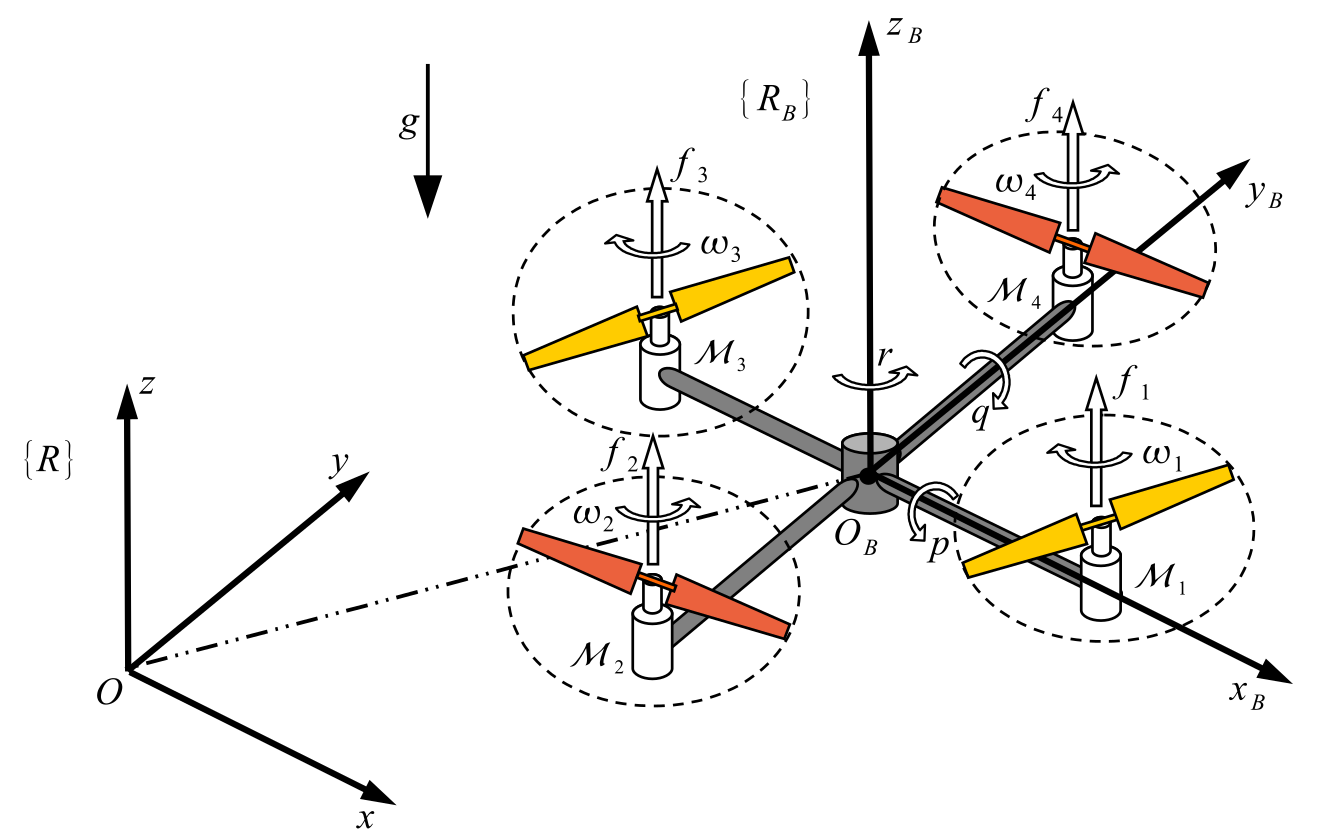
\includegraphics[width=0.7\linewidth]{Images/Quad_model}
	\caption{Quadrotor scheme used for the development of the mathematical model.}
	\label{fig:quadmodel}
\end{figure}

A quadrotor consists of four rotors on which propellers are fixed. The rotors are positioned at the ends of a X-shaped frame. The front and rear motors $\mathcal{M}_1$ and $\mathcal{M}_3$ spin in the clockwise direction, the other two motors $\mathcal{M}_2$ and $\mathcal{M}_4$ spin in the counter-clockwise direction, as shown in fig.\ref{fig:quadmodel}.

The mathematical is based on three assumptions:
\begin{itemize}
	\item the quadrotor structure is symmetrical. This means that the inertias along the longitudinal axis and the lateral one are equal;
	\item propellers are considered rigid: no blade flapping;
	\item drag is assumed linear.
\end{itemize}

As one can see in fig.\ref{fig:quadmodel}, we define two reference frames:
\begin{itemize}
	\item the first one, representing the Earth frame: $ \{R\}\{O, x, y, z\} $;
	\item the second, representing the body-fixed frame: $ \{R_b\}\{O_b, x_b, y_b, z_b\} $.
\end{itemize}

The body fixed frame is connected to $ \{R\} $ by a position vector $ [x, y, z] $, which describes the center of gravity in $ \{R_b\} $ relative to $ \{R\} $, and by a vector of angles $ [\phi, \theta, \psi] $, i.e. the roll, pitch and yaw angles, which represent the orientation of the body frame w.r.t the Earth frame.

The rotation along roll and pitch angles are constrained\footnote{Consequently, no acrobatic maneuvers and inverted flight are allowed.}:
\begin{equation*}
	(-\frac{\Pi}{2}<\phi<\frac{\Pi}{2}), \qquad (-\frac{\Pi}{2}<\theta<\frac{\Pi}{2})
\end{equation*}
while the yaw angle $ \psi $ is unconstrained.

The inertia matrix in the body frame is:
\begin{equation*}
	\mathbf{I}=
	\begin{bmatrix}
	I_{xx} & 0 & 0 \\
	0 & I_{yy} & 0 \\
	0 & 0 & I_{zz} 
	\end{bmatrix}
\end{equation*}
and we can assume $ I_{xx} = I_{yy} $ due to the symmetric structure.

The  dynamic model of the quadrotor is defined starting from the forces acting on it:
\begin{itemize}
	\item the generalized forces, computed starting from the forces generated by every rotor;
	\item the drag force, proportional to the linear and angular velocity;
	\item the weight, applied to the center of gravity along the negative $ z $ axis of Earth frame.
\end{itemize}

The complete model of a quadrotor is:

\begin{equation}
\begin{cases}
\ddot{x} = \frac{1}{m}[(C_{\phi}S_{\theta}C_{\psi} + S_{\phi}S_{\psi})u_f-k_t \dot{x}] \\
\ddot{y} = \frac{1}{m}[(C_{\phi}S_{\theta}S_{\psi} - S_{\phi}C_{\psi})u_f-k_t \dot{y}] \\
\ddot{z} = \frac{1}{m}[(C_{\phi}C_{\theta})u_f- mg - k_t \dot{z}] \\
\dot{p} = \frac{1}{I_{xx}}[-k_r p - qr(I_{zz}-I_{yy})+\tau_p]  \\
\dot{q} = \frac{1}{I_{yy}}[-k_r q - pr(I_{xx}-I_{zz})+\tau_q]  \\
\dot{r} = \frac{1}{I_{zz}}[-k_r r - pq(I_{yy}-I_{xx})+\tau_r]  \\
\dot{\phi} = p + q S_{\phi}T_{\theta} + r C_{\phi}T_{\theta} \\
\dot{\theta} = q C_{\phi} - rS_{\phi} \\
\dot{\psi} = \frac{1}{C_{\theta}}[qS_{\phi}+rC_{\phi}]
\end{cases}
\label{quad_model_eqs}
\end{equation}

where:
\begin{itemize}
	\item $ p, \ q, \ r $ = roll, pitch and yaw velocity, $ rad/s $;
	\item $ k_r $ = rotational drag, $ N \cdot m \cdot s  $;
	\item $ k_t $ = linear drag, $ N \cdot m/s  $;
	\item $ m $ = quadrotor mass, $ kg $;
	\item $ g $ = gravity acceleration, $ 9.81 m/s^2 $
	\item $ u_f $ = total upward lift force, $ N $;
	\item $ \tau_p, \ \tau_q, \ \tau_r $ = torque around roll, pitch and yaw axis, $ N\cdot m $;
\end{itemize}
and $ C(\cdot), \ S(\cdot), \ T(\cdot) $ stand for $ cos(\cdot), \ sin(\cdot), \ tan(\cdot) $.

In \eqref{quad_model_eqs} the system inputs are the generalized forces $ u_f, \ \tau_p, \ \tau_q, \ \tau_r $, while the real actuation is given by the four motors forces $ f_1, \ f_2, \ f_3, \ f_4 $.

The relation between these is given by:
\begin{equation}
	\begin{bmatrix}
	u_f \\ \tau_p \\ \tau_q \\ \tau_r
	\end{bmatrix} = 
	\begin{bmatrix}
	 1 & 1 & 1 & 1 \\
	 0 & -l & 0 & l \\
	 -l & 0 & l & 0 \\
	 d & -d & d & -d
	\end{bmatrix}
	\begin{bmatrix}
	f_1 \\ f_2 \\ f_3 \\ f_4
	\end{bmatrix}
	\label{forceTorqueMapping}
\end{equation}
in which:
\begin{itemize}
	\item $ d $ = the ratio between drag and thrust coefficients of the rotor, $ m $;
	\item $ l $ = the arm length, $ m $.
\end{itemize}

Every $ f_i $ is applied to the center of the \emph{i}-rotor and is directed along the $ z_b $ axis. From \eqref{forceTorqueMapping} is clear that the total lift $ u_f $ is equal to $ \sum_i f_i $. The torques around roll and pitch axis are due to the torque of every motor, $ l\cdot f_i $. The torque around the yaw axis, instead, is caused by unbalanced clockwise and counterclockwise drag reaction torques. 

\section{Controller architecture}

As mentioned in the introduction, usually the control strategy of a quadrotor is based on a double-loop architecture: an outer controller that takes the reference trajectory and computes the attitude angles needed to achieve it and an inner controller whose task is to regulate these attitude angles acting on the generalized forces.

In case of failure of one motor, the quadrotor loses the capability to control one of the variable among roll, pitch, yaw and altitude, or, in other words, it loses the ability to control independently the three torques required for the control of the attitude.

The controller developed in \cite{lanzon2014flight} is based on the assumption that one rotor has failed, while the others are full working. In  this case, the controller task is to safely landing, instead of achieving the mission.

In \cite{lanzon2014flight} and \cite{freddi2011feedback}, the authors claim that controlling a subset of attitude dynamics is enough to make the vehicle fly, although it is spinning around the yaw axis. The most important variables to control are roll, pitch and altitude: roll and pitch are essential because a change in their values results in a horizontal displacement; while altitude is fundamental in order to avoid collision with the ground.

For these reasons the yaw state is the one sacrificed.

Using only three rotors, the unbalance in propeller drag makes the quadrotor spinning around the yaw axis. To make the quadrotor increase its altitude it is needed to increase the total lift $ u_f $: the consequence is an acceleration around the yaw axis. The rotational speed around the vertical axis and the altitude variation depends on the same input. 

For this reason the inner control loop is designed to control the roll and pitch angles and yaw velocity, while the outer controller sets the desired values of these variables. In particular, the desired altitude is obtained changing the set point of the yaw velocity.

%Mettere che l'outer controller lavora piu lentmente dell'inner.

To control the quadrotor all the states must be accessible.

\begin{figure}
	\centering
	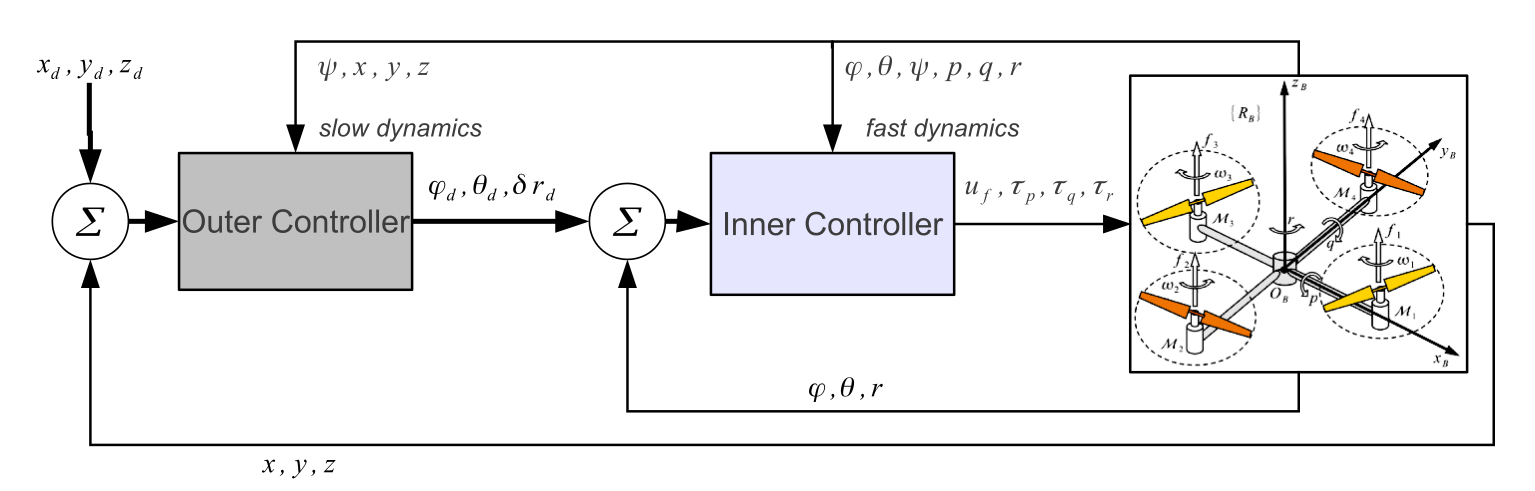
\includegraphics[width=0.9\linewidth]{Images/ControlScheme}
	\caption{The double-loop architecture in case of actuator loss.}
	\label{fig:controlscheme}
\end{figure}

\subsection{Quadrotor model in case of rotor loss}

\subsubsection{Control inputs constraints}

In case of failure of rotor $\mathcal{M}_2$ the mapping \eqref{forceTorqueMapping} becomes:
\begin{equation}
\begin{bmatrix}
u_f \\ \tau_q \\ \tau_r
\end{bmatrix} = 
\begin{bmatrix}
1 & 1 & 1 \\
-l & l & 0 \\
d  & d & -d
\end{bmatrix}
\begin{bmatrix}
f_1 \\ f_3 \\ f_4
\end{bmatrix}
\label{forceTorqueMappingFailure}
\end{equation}

In this case the control inputs are $ u_f, \ \tau_q, \ \tau_r $, while $ \tau_p $ is no longer used as input.

The constraints on the real inputs $ f_i $ are:
\begin{equation}
	\begin{cases}
	f_i \geq 0 \\
	f_i \leq f_{max} 
	\end{cases} \qquad i = 1,3,4
	\label{constraints}
\end{equation}

We need to obtain the constraints on the control inputs $ u_f, \ \tau_q, \ \tau_r $. From \eqref{forceTorqueMappingFailure}
\begin{equation}
	\begin{bmatrix}
	f_1 \\ f_3 \\ f_4
	\end{bmatrix} = \frac{1}{4} 
	\begin{bmatrix}
	1 & -2/l & l/d \\
	1 & 2/l & l/d \\
	2 & 0 & -2/d
	\end{bmatrix}
	\begin{bmatrix}
	u_f \\ \tau_q \\ \tau_r
	\end{bmatrix}
\end{equation}
and imposing the first of \eqref{constraints}  
\begin{equation}
	\begin{cases}
	u_f - \dfrac{2 \tau_q}{l} + \dfrac{\tau_r}{d} \geq 0 \\
	u_f + \dfrac{2 \tau_q}{l} + \dfrac{\tau_r}{d} \geq 0 \\
	2 u_f - \dfrac{2 \tau_r}{l} \geq 0
	\end{cases} \quad
	\Rightarrow \qquad
	\begin{cases}
	|\tau_q| \leq \dfrac{l}{2}(u_f + \dfrac{\tau_r}{d}) \\
	|\tau_r| \leq d\cdot u_f
	\end{cases}
\end{equation}

to which we add:

\begin{equation}
	u_f \leq 3 \cdot f_{max}
\end{equation}
from the second of \eqref{constraints}.

\subsubsection{State-space model}

The state vector is chosen as:
\begin{align*}
	\mathbf{x} \ &= \ [&x_1 &\ &x_2 &\ &x_3 &\ &x_4 &\ &x_5 &\ &x_6 &\ &x_7 &\ &x_8 &\ &x_9 &\ &x_{10} &\ &x_{11} &\ &x_{12} \ ]^T \\
	&= \ [&\phi &\ &\theta &\ &\psi &\ &p &\ &q &\ &r &\ &x &\ &y &\ &z &\ &\dot{x} &\ &\dot{y} &\ &\dot{z} \ ]^T
\end{align*}
and the input vector is:
\begin{equation}
	\mathbf{u} \ = \ [ \ u_1 \quad u_2 \quad u_3 \ ]^T \ = \ [ \ u_f \quad \tau_q \quad \tau_r \ ]^T
\end{equation}

Since $ f_2 = 0 $ and \eqref{forceTorqueMapping}, the neglected input can be expressed as $ \tau_p = l \cdot f_4 $, and hence:

\begin{equation}
	f_4 = \dfrac{1}{2}( u_1 - \dfrac{u_3}{d}) \qquad \Rightarrow \qquad \tau_p = \dfrac{l}{2}(u_1 -\dfrac{u_3}{d})
\end{equation}

The complete quadrotor model \eqref{fig:quadmodel} in state-space form can be written as:
\begin{subequations}
\begin{align}
	\dot{\phi} & = \dot{x}_1 = x_4 + x_5 S_{x_1} T_{x_2} + x_6 C_{x_1} T_{x_2} \\
	\dot{\theta} & = \dot{x}_2 = x_5 C_{x_1} \\
	\dot{\psi} & =  \dot{x}_3 = \dfrac{1}{C_{x_2}} [ x_5 S_{x_1} + x_6 C_{x_1}] \\
	\dot{p} & = \dot{x}_4 = \dfrac{1}{I_{xx}}[-k_r x_4 - x_5 x_6 (I_{zz} - I_{xx}) + \dfrac{l}{2} (u_1 -\dfrac{u_3}{d})] \label{rollDynamics} \\
	\dot{q} & = \dot{x}_5 = \dfrac{1}{I_{xx}}[-k_r x_4 - x_5 x_6 (I_{zz} - I_{xx}) + u_2] \label{pitchDynamics} \\
	\dot{r} & = \dot{x}_6 = \dfrac{1}{I_{xx}}(-k_r x_6 + u_3) \label{yawDynamics}\\
	\dot{x} & = \dot{x}_7 = x_{10} \\
	\dot{y} & = \dot{x}_8 = x_{11} \\
	\dot{z} & = \dot{x}_9 = x_{12} \\
	\ddot{x} & = \dot{x}_{10} = \dfrac{C_{x_1} S_{x_2} C_{x_3} + S_{x_1} S_{x_3}}{m} u_1 - \dfrac{k_t}{m}x_{10} \\
	\ddot{y} & = \dot{x}_{11} = \dfrac{C_{x_1} S_{x_2} S_{x_3} - S_{x_1} C_{x_3}}{m} u_1 - \dfrac{k_t}{m}x_{11} \\
	\ddot{z} & = \dot{x}_{12} = \dfrac{1}{m} [u_1 C_{x_1} C_{x_2} - k_t x_{12} - m g]
\end{align}
\label{completeQuadModel}
\end{subequations}
where in \eqref{yawDynamics} $ I_{xx} $ is chosen to be equal to $ I_{yy} $ due to the symmetry of the vehicle.

\subsection{Outer control loop}

The horizontal motion depends on the projection of the thrust vector on the $ (x,y) $ plane. The direction of this vector depends on the roll and pitch angles.

The task of the outer control is to generate the right values of roll and pitch angles to reach a desired position in the Earth frame. The vertical dynamics, on the other side, is controlled by the variation of the yaw velocity $ r $ around a working point\footnote{We will discuss this working point in the inner control loop.}.

Assuming that the inner controller is stabilizing the state near the equilibrium:
\begin{equation}
	x_1=\phi \rightarrow \phi_d, \qquad x_2=\theta \rightarrow \theta_d, \qquad x_6=r \rightarrow r_d
\end{equation}
the chosen desired values $ \phi_d $ and $ \theta_d $ must be small.

We compute the inputs at the steady state:
\begin{itemize}
	\item from \eqref{pitchDynamics}:
	\begin{equation}
	\dot{q}  = \dot{x}_5 = \dfrac{1}{I_{xx}}[-k_r x_4 - x_5 x_6 (I_{zz} - I_{xx}) + u_2] = 0 \qquad \Rightarrow \qquad u_2 \rightarrow 0 
	\end{equation}
	\item from \eqref{yawDynamics}:
	\begin{equation}
	\dot{r} = \dot{x}_6 = \dfrac{1}{I_{xx}}(-k_r x_6 + u_3) = 0 \qquad \Rightarrow \qquad u_3 \rightarrow x_{6d} k_r
	\end{equation}
	\item from \eqref{rollDynamics}:
	\begin{equation}
	\begin{split}
	\dot{p} = \dot{x}_4 = &\dfrac{1}{I_{xx}}[-k_r x_4 - x_5 x_6 (I_{zz} - I_{xx}) + \dfrac{l}{2} (u_1 -\dfrac{u_3}{d})] = 0 \\ 
	&\Rightarrow \qquad u_1 \rightarrow \dfrac{u_3}{d}= \dfrac{x_{6d} k_r}{d}
	\end{split}
	\end{equation}
\end{itemize}

Using the assumption of small angles for $ \phi_d $ and $ \theta_d $, the model relative to the outer control loop can be expressed as:
\begin{subequations}
	\begin{align}
	\dot{x}_7 & = x_{10} \\
	\dot{x}_8 & = x_{11} \\
	\dot{x}_9 & = x_{12} \\
	\dot{x}_{10} & = \dfrac{ x_{2d} C_{x_3} + x_{1d} S_{x3} }{m} \overbracket{\dfrac{k_r}{d} x_{6d}}^{u_1} -\dfrac{k_t}{m} x_{10} \\
	\dot{x}_{11} & = \dfrac{ x_{2d} S_{x_3} + x_{1d} C_{x3} }{m} \overbracket{\dfrac{k_r}{d} x_{6d}}^{u_1} -\dfrac{k_t}{m} x_{11} \\
	\dot{x}_{12} & = \dfrac{1}{m} \Big[{\overbracket{\dfrac{k_r}{d} x_{6d}}^{u_1}} - k_t x_{12} - mg \Big]
	\end{align}
	\label{outerModel}
\end{subequations}
 
The state of the outer control loop is chosen as:
\begin{align*}
\mathbf{\tilde{x}} \ &= \ [ \ \tilde{x}_1 \quad \tilde{x}_2 \quad \tilde{x}_3 \quad \tilde{x}_4 \quad \tilde{x}_5 \quad \tilde{x}_6 \ ]^T \\
&= \ [ \ x_7 \quad x_8 \quad x_9 \quad x_{10} \quad x_{11} \quad x_{12} \ ]^T
\end{align*}

While the control inputs vector is chosen so as to linearize the state-space equations:
\begin{equation}
	\mathbf{\tilde{u}} = [\tilde{u}_1 \quad \tilde{u}_2 \quad \tilde{u}_3] = \Big[ \dfrac{k_r x_{6d}}{dm}  x_{1d} \quad  \dfrac{k_r x_{6d} }{dm} x_{2d} \quad  \dfrac{k_r x_{6d}}{dm} \Big]
	\label{OuterInputs}
\end{equation}

The equations \eqref{outerModel} can be rewritten as:
\begin{subequations}
	\begin{align}
		 \dot{\tilde{x}}_1 & = \tilde{x}_4 \\
		 \dot{\tilde{x}}_2 & = \tilde{x}_5 \\
		 \dot{\tilde{x}}_3 & = \tilde{x}_6 \\
		 \dot{\tilde{x}}_4 & = C_\psi \tilde{u}_2 + S_\psi \tilde{u}_1 - \dfrac{k_t}{m} \tilde{x}_4 \\
		 \dot{\tilde{x}}_5 & = S_\psi \tilde{u}_2 - C_\psi \tilde{u}_1 - \dfrac{k_t}{m} \tilde{x}_5 \\
		 \dot{\tilde{x}}_6 & = \tilde{u}_3 - \dfrac{k_t}{m} \tilde{x}_6 - g
	\end{align}
	\label{outerControl_}
\end{subequations}

The dynamics of longitudinal ($ \tilde{x}_1, \tilde{x}_4 $) and lateral ($ \tilde{x}_2, \tilde{x}_5 $) motion are decoupled from the altitude one ($ \tilde{x}_3,  \tilde{x}_6 $).

The vertical dynamics is linear and can be controlled with any standard control technique. 

$ \tilde{x}_1, \tilde{x}_2, \tilde{x}_4, \tilde{x}_5 $ have nonlinear dynamics that depend on the yaw angle $ \psi $.

To linearize the nonlinear dynamics we use the following control inputs:
\begin{equation}
	\begin{bmatrix}
	\tilde{u}_1 \\ \tilde{u}_2
	\end{bmatrix} = 
	\begin{bmatrix}
	S_{\psi} & -C_{\psi} \\
	C_{\psi} & S_{\psi} 
	\end{bmatrix}
	\begin{bmatrix}
	\tilde{\tilde{u}}_1 \\ \tilde{\tilde{u}}_2
	\end{bmatrix}
	\label{rotation_matrix_outer}
\end{equation}
where the new control inputs $ \tilde{\tilde{u}}_1, \tilde{\tilde{u}}_2 $ are premultiplied by the rotation matrix.

Substituting $ \tilde{\tilde{u}}_1, \tilde{\tilde{u}}_2 $ in \eqref{outerControl_}, the lateral and longitudinal dynamics become linear and decoupled and thus can be controlled with a simple linear control technique.

\begin{subequations}
	\begin{align}
		\dot{\tilde{x}}_4 & = \tilde{\tilde{u}}_1 - \dfrac{k_t}{m} \tilde{x}_4 \\
		\dot{\tilde{x}}_5 & = \tilde{\tilde{u}}_2 - \dfrac{k_t}{m} \tilde{x}_5
	\end{align}
\end{subequations}

The control inputs are chosen as:
\begin{equation}
	u_i = \ddot{x}_i + 2\xi_{out}c_{out} \dot{e}_i + c_{out}^2 e_i 
\end{equation}
where $ \ddot{x}_i $ is the feed-forward term, $ e_i = x_{di} - x_i $ is the error. $ \xi_{out} $ and $ c_{out} $ are positive constants. 

$ c_{out} $ represents the natural frequency of the dynamical system and must be small: actually the outer control loop must be slower than the inner control loop. 

From \eqref{OuterInputs} and having computed $ \tilde{u}_1, \tilde{u}_2, \tilde{u}_3 $ we have the desired values of $ [\phi_d, \theta_d, r_d]=[x_{1d}, x_{2d}, x_{6d}] $ to use as set points for the inner control loop\footnote{Note that, at equilibrium, $ \tilde{u}_3 \rightarrow g $ and hence $ r_d \rightarrow \dfrac{mgd}{k_r} $, while $ \phi_d $ and $ \theta_d $ remain small angle.}. 

%inserire la control law???

\subsection{Inner control loop}

The inner control loop task is to control the dynamics of the attitude angles and the yaw velocity.

The equations in \eqref{completeQuadModel} relative to $ \psi, \theta, p, q, r $ are expressed such that the origin of the system is an equilibrium point when the inputs are equal to zero.

The state is\footnote{In the previous section we have seen that at equilibrium $ r \rightarrow \dfrac{mgd}{k_r} $. }:
\begin{equation}
	\mathbf{\hat{x}} = [ \ \hat{x}_1 \quad \hat{x}_2 \quad \hat{x}_3 \quad \hat{x}_4 \quad \hat{x}_5 \ ] = \Big[ \ x_1 \quad x_1 \quad x_2 \quad x_3 \quad x_4 \quad (x_6-\dfrac{mgd}{k_r}) \ \Big]	
\end{equation}
while the inputs are:
\begin{equation}
	\mathbf{\hat{u}} = [ \ \hat{u}_1 \quad \hat{u}_2 \quad \hat{u}_3 \ ] = [ \ (u_1 -mg) \quad u_2 \quad (u_3 - mgd) \ ]
\end{equation}
reminding that $ [u_1, u_2, u_3] = [u_f, \tau_q, \tau_r ]  $.

The $ \mathbf{\hat{x}} $ dynamics are given by:
\begin{equation}
	\mathbf{\dot{\hat{x}}=\hat{f}(\hat{x})+\hat{G}(\hat{x})\hat{u}}
\end{equation}
and the output is:
\begin{equation}
	\mathbf{\hat{y}}= [ \ \hat{h}_1 \quad \hat{h}_2 \quad \hat{h}_3 \ ] = [ \ \hat{x}_1 \quad \hat{x}_2 \quad \hat{x}_5 \ ]
\end{equation}
where:
\renewcommand{\arraystretch}{1.6}
\begin{equation}
	\mathbf{\hat{f}(\hat{x})}=
	\begin{bmatrix}
	\hat{x}_3 + \hat{x}_4 S_{\hat{x}_1} T_{\hat{x}_2} + (\hat{x}_5 + \dfrac{mgd}{k_r}) C_{\hat{x}_1} T_{\hat{x}_2} \\
	\hat{x}_4 C_{\hat{x}_1} - (\hat{x}_5 + \dfrac{mgd}{k_r}) s_{\hat{x}_1}  \\
	\dfrac{1}{I_{xx}} [-k_r \hat{x}_3 - \hat{x}_4(\hat{x}_5 + \dfrac{mgd}{k_r}) (I_{zz} - I_{yy}) ] \\
	\dfrac{1}{I_{yy}} [-k_r \hat{x}_4 - \hat{x}_3(\hat{x}_5 + \dfrac{mgd}{k_r}) (I_{xx} - I_{zz})] \\
	\dfrac{1}{I_{zz}} (-k_r \hat{x}_5)
	\end{bmatrix}
\end{equation}
\renewcommand{\arraystretch}{1}
\begin{equation}
	\mathbf{\hat{G}(\hat{x})} =
	\begin{bmatrix}
	0 & 0 & 0 \\
	0 & 0 & 0 \\
	\dfrac{l}{2I_{xx}} & 0 & -\dfrac{l}{2I_{xx}} \\
	0 & \dfrac{1}{I_{xx}} & 0 \\
	0 & 0 & \dfrac{1}{I_{zz}}	
	\end{bmatrix}
\end{equation}


\subsubsection{Feedback Linearization}

The system fulfills the condition for the feedback linearization:
\begin{itemize}
	\item the relative degrees are $ r_1 = 2 $ ($ h_1 $), $ r_2 = 2 $ ($ h_2 $), $ r_3 = 1 $ ($ h_5 $). $ r_1 + r_2 + r_3 = n = 5 $, the dimension of the state vector;
 
	\item the decoupling matrix:
	\begin{equation}
	\mathbf{M(\hat{x})} = 
	\begin{bmatrix}
	\dfrac{l}{2I_{xx}} & \dfrac{S_{\hat{x}_1} T_{\hat{x}_2}}{I_{xx}} & \dfrac{C_{\hat{x}_1}T_{\hat{x}_2}}{I_{zz}} -\dfrac{l}{2dI_{xx}} \\
	0 & \dfrac{C_{\hat{x}_1}}{I_{xx}} & -\dfrac{S_{\hat{x}_1}}{I_{zz}} \\
	0 & 0 & \dfrac{1}{I_{zz}} 
	\end{bmatrix}
	\end{equation}
	is always invertible.
\end{itemize}

We can compute the linearizing input as:
\begin{equation}
	\mathbf{u(x,v) = \alpha(x)+\beta(x)*v}
	\label{LinearizingControlLaw}
\end{equation}
where $ \alpha(\mathbf{x}) = [ \ \alpha_1(\mathbf{x}) \quad \alpha_2(\mathbf{x}) \quad \alpha_3(\mathbf{x}) \ ] $ is:
\begin{equation}
	\begin{split}
	\alpha_1(\mathbf{x}) = & \
	( \ 2 d k_r^3 \hat{x}_3  C_{\hat{x}_1}  C_{\hat{x}_2}^2 + k_r^3 l \hat{x}_5  C_{\hat{x}_1}  C_{\hat{x}_2}^2 - 2 I_{xx} d k_r^2 \hat{x}_4^2 S_{\hat{x}_1} 
	- 4 I_{xx} d k_r^2 \hat{x}_4 \hat{x}_5  C_{\hat{x}_1}^3 \\
	&+ 2 I_{xx} d^3 g^2 m^2  C_{\hat{x}_1}^2 S_{\hat{x}_1} - 2 I_{xx} d k_r^2 \hat{x}_4^2  C_{\hat{x}_1}^2 S_{\hat{x}_1} + 2 I_{xx} d k_r^2 \hat{x}_4^2  C_{\hat{x}_2}^2 S_{\hat{x}_1} \\
	& + 2 I_{xx} d k_r^2 \hat{x}_5^2  C_{\hat{x}_1}^2 S_{\hat{x}_1} - 4 I_{xx} d^2 g k_r m \hat{x}_4  C_{\hat{x}_1}^3 - 2 I_{xx} d k_r^2 \hat{x}_3 \hat{x}_4  C_{\hat{x}_2} S_{\hat{x}_2} + 2 I_{zz} d k_r^2 \hat{x}_4 \hat{x}_5  C_{\hat{x}_1}  C_{\hat{x}_2}^2 \\
	& + 2 I_{zz} d^2 g k_r m \hat{x}_4  C_{\hat{x}_1}  C_{\hat{x}_2}^2 + 4 I_{xx} d^2 g k_r m \hat{x}_5  C_{\hat{x}_1}^2 S_{\hat{x}_1} \ )/( \ d k_r^2 l  C_{\hat{x}_1}  C_{\hat{x}_2}^2 \ )
	\end{split}
\end{equation}

\begin{equation}
	\begin{split}
	\alpha_2(\mathbf{x}) = & \
	(I_{xx} (C_{\hat{x}_1} ( \hat{x}_5 + (d g m)/k_r) + \hat{x}_4 S_{\hat{x}_1}) (\hat{x}_3 + C_{\hat{x}_1} T_{\hat{x}_2}
	( \hat{x}_5 + (d g m)/k_r) + \hat{x}_4 S_{\hat{x}_1} T_{\hat{x}_2}) \\
	&+ C_{\hat{x}_1} (k_r \hat{x}_4 + \hat{x}_3 (\hat{x}_5 + (d g m)/k_r) (I_{xx} - I_{zz})))/I_{xx} \\
	&- (k_r \hat{x}_5 S_{\hat{x}_1})/I_{zz}))/C_{\hat{x}_1} + (I_{xx} k_r \hat{x}_5 S_{\hat{x}_1})/(I_{zz} C_{\hat{x}_1})
	\end{split}
\end{equation}

\begin{flalign}
\alpha_3(\mathbf{x}) = k_r \hat{x}_5 &&
\end{flalign}
and $ \beta(\mathbf{x}) $:
\begin{equation}
	\beta(\mathbf{x}) = 
	\begin{bmatrix}
	2 \dfrac{I_{xx}}{l} & -2 \dfrac{I_{xx} T_{\hat{x}_1} T_{\hat{x}_2}}{l} & - \dfrac{2 I_{xx} T_{\hat{x}_2}}{l C_{\hat{x}_1}} + \dfrac{I_{zz} T_{\hat{x}_1}}{d} \\
	0 & \dfrac{I_{xx}}{C_{\hat{x}_1}} & I_{xx} T_{\hat{x}_1} \\
	0 & 0 & I_{zz}
	\end{bmatrix}
\end{equation}

The \eqref{LinearizingControlLaw} leads to the canonical Brunowski form:
\begin{equation}
	\mathbf{\dot{x}_c = A_c x_c + B_c v}
\end{equation}
\renewcommand{\arraystretch}{1}
%\setlength{\arraycolsep}{8pt}
\begin{equation}
	\mathbf{A_c} = 
	\begin{bmatrix}
	0 & 0 & 1 & 0 & 0 \\
	0 & 0 & 0 & 1 & 0 \\
	0 & 0 & 0 & 0 & 0 \\
	0 & 0 & 0 & 0 & 0 \\
	0 & 0 & 0 & 0 & 1	
	\end{bmatrix} \qquad
	\mathbf{B_c} = 
	\begin{bmatrix}
	0 & 0 & 0 \\
	0 & 0 & 0 \\
	1 & 0 & 0 \\
	0 & 1 & 0 \\
	0 & 0 & 1
	\end{bmatrix}
\end{equation}
and the state vector $ \mathbf{x_c} = [ \ \hat{h}_1 \quad \hat{h}_2 \quad \dot{\hat{h}}_1 \quad \dot{\hat{h}}_2 \quad \hat{h}_3 \ ] = [ \ \hat{x}_1 \quad \hat{x}_2 \quad \dot{\hat{x}}_1 \quad \dot{\hat{x}}_2 \quad \hat{x}_5 \ ] $.

The linear input $ \mathbf{v} $ is chosen to regulate the state variables $ \hat{x}_1, \hat{x}_2, \hat{x}_5 $ to the desired values, coming from the outer control loop.

Usually, the desired roll and pitch angles and the variation of yaw velocity are chosen to converge to zero. As a result, the roll velocity $ p $ and the pitch velocity $ q $ will converge to zero and the yaw velocity $ r $ will converge to the constant value $ mgd / k_r $. 

\section{Simulations}

In this section are presented the behaviors of the outer control loop, the inner control loop and then of the overall system when both the inner and the outer control loops are activated. The model parameters used in the simulations are in Table.\ref{Quadrotor and parameters}.

\begin{table}[H]
	\centering
	\begin{tabular}{c c c}
		\toprule
		Constant & Value & Description \\
		\midrule 
		$m$  & $0.5$ kg & Quadrotor mass \\
		$g$  & $9.81$ m/ s\textsuperscript{2}  & Gravity acceleration \\
		$I_{xx}$  & $5.9\cdot 10^{-3}$ kg m\textsuperscript{2} & Inertia coefficient along x axis \\
		$I_{yy}$  & $5.9\cdot 10^{-3}$ kg m\textsuperscript{2} & Inertia coefficient along y axis \\
		$I_{zz}$  & $1.16\cdot 10^{-3}$ kg m\textsuperscript{2} & Inertia coefficient along z axis \\
		$l$  & $0.255$ m & Distance between rotor and c.g. \\
		$d$  & $2.4\cdot 10^{-3}$ kg m\textsuperscript{2} & Blade drag / thrust ratio \\
		$k_r$  & $0.1$ N m s & Rotational drag \\
		$k_t$  & $0.1$ N s/m & Linear drag \\
%		$x_{10}$  & $0$ m/s & $\dot{x}$ \\
%		$x_{11}$  & $0$ m/s & $\dot{y}$ \\
%		$x_{12}$  & $0$ m/s & $\dot{z}$ \\
		\bottomrule
	\end{tabular}
	\caption{Quadrotor and controller parameters.}
	\label{Quadrotor and parameters}
\end{table}

\subsection*{Outer control loop}

In the first simulation only the outer control loop is activated. Specifically we want to regulate the position from the initial condition, expressed in Table \ref{InitCondOuter}, to the origin of the Earth frame.

\begin{table}[H]
	\centering
	\begin{tabular}{c c c}
		\toprule
		Variable & Value & Description \\
		\midrule 
		$\tilde{x}_1$  & $ 2 $ m & $x$ \\
		$\tilde{x}_2$  & $3$ m & $y$ \\
		$\tilde{x}_3$  & $4$ m & $z$ \\
		$\tilde{x}_4$  & $0$ m/s & $\dot{x}$ \\
		$\tilde{x}_5$  & $0$ m/s & $\dot{y}$ \\
		$\tilde{x}_6$  & $0$ m/s & $\dot{z}$ \\
		\bottomrule
	\end{tabular}
	\caption{Initial conditions for the outer control loop simulation.}
	\label{InitCondOuter}
\end{table}

Since we don't want the initial error to be too large (and hence, the inputs), a module has been used that computes a cubic trajectory that lasts $ 50 $ seconds.

We set a constant spinning velocity equal to $ 0.3 $ rad/s. As shown in fig.\ref{fig:outercontrolpos} the outer control loop tracks the reference trajectory perfectly. The reference values coming out from the outer control loop inputs in eq.\eqref{OuterInputs} are shown in fig.\ref{fig:ReferenceValues}.

\begin{figure}[H]
		\centering
		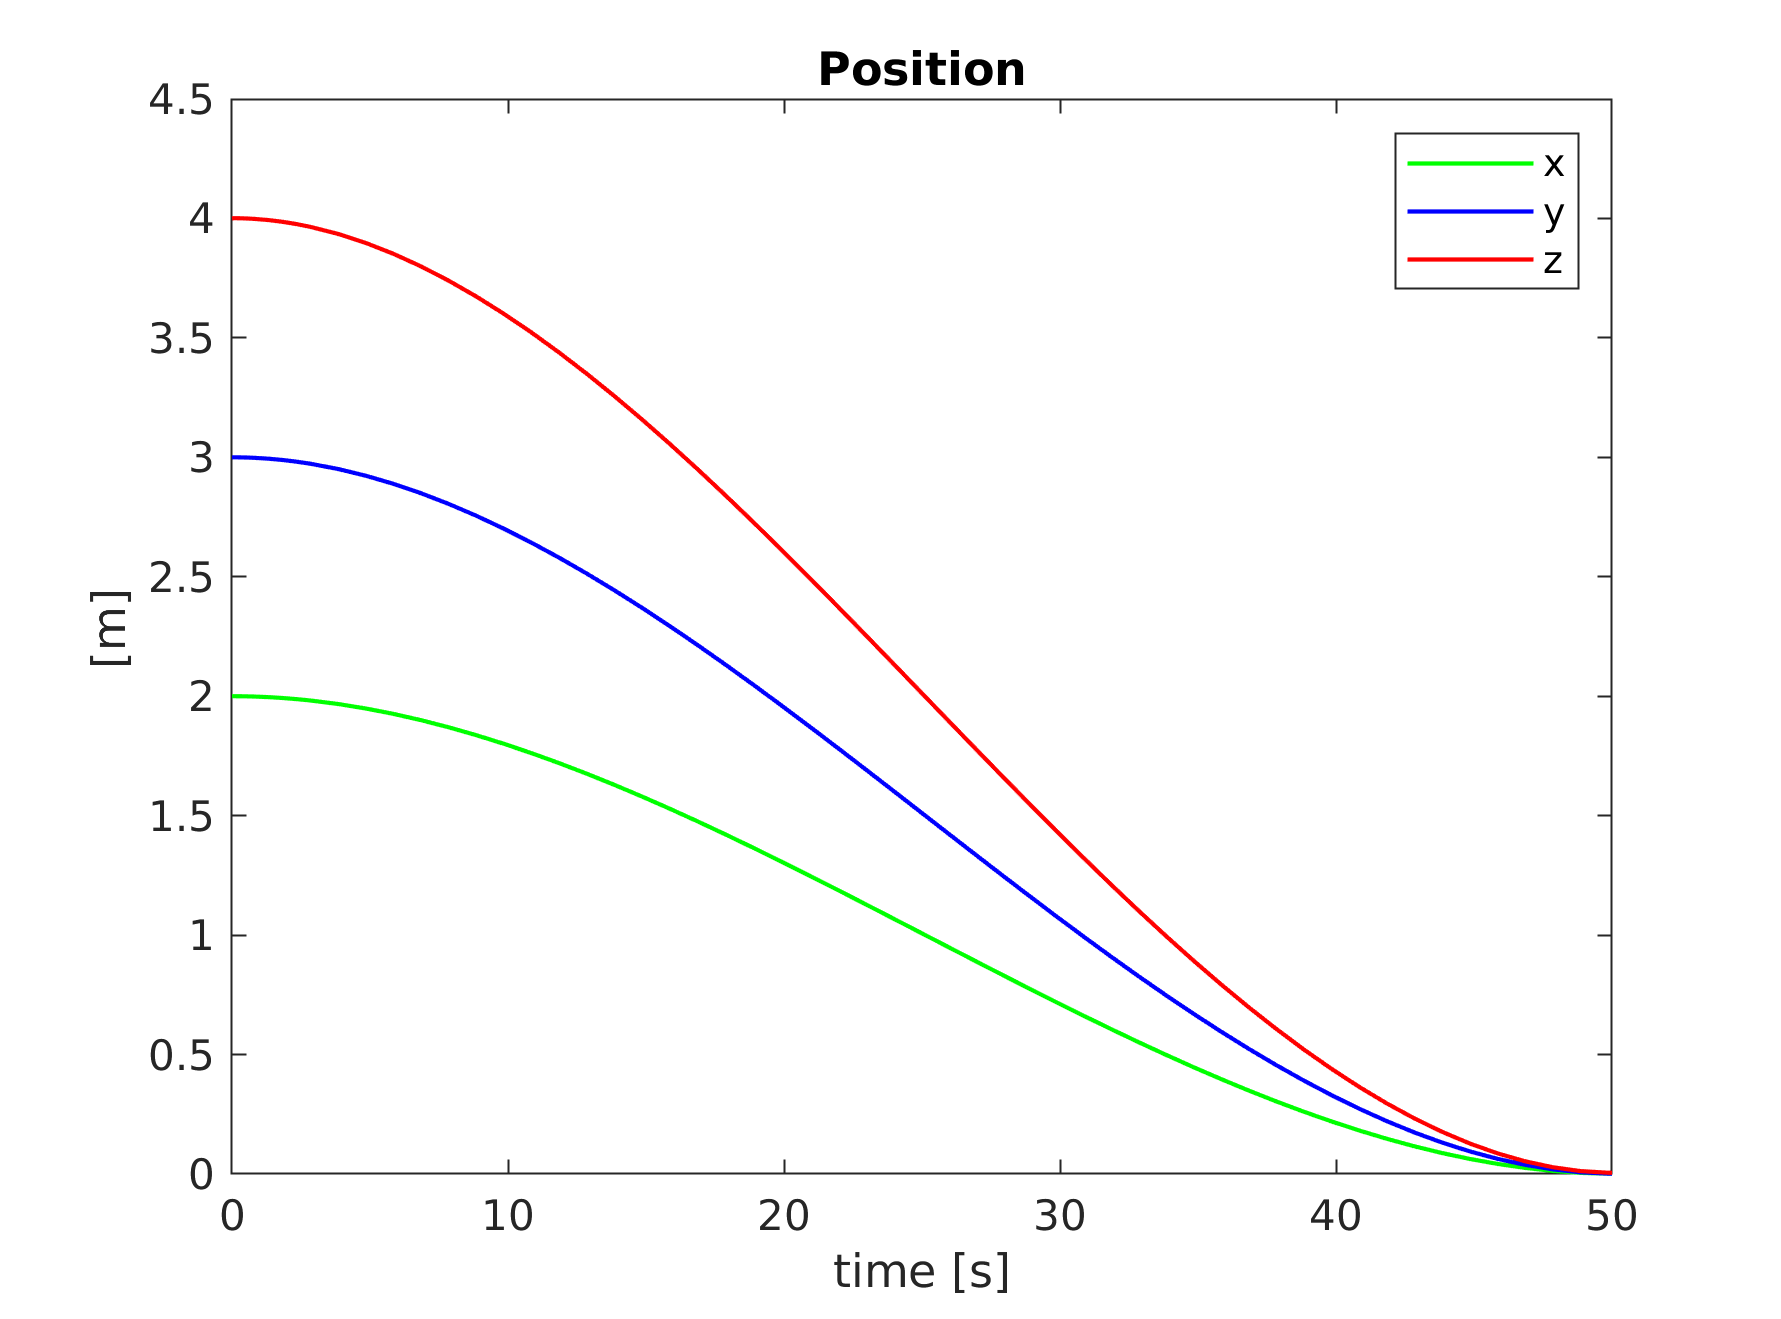
\includegraphics[width=0.6\linewidth]{Images/PositionOuter.png}
		\caption{Position in the Earth frame.}
		\label{fig:outercontrolpos}	
\end{figure} 

\begin{figure}[h]
	\begin{subfigure}[h!]{0.5\linewidth}
		\centering
		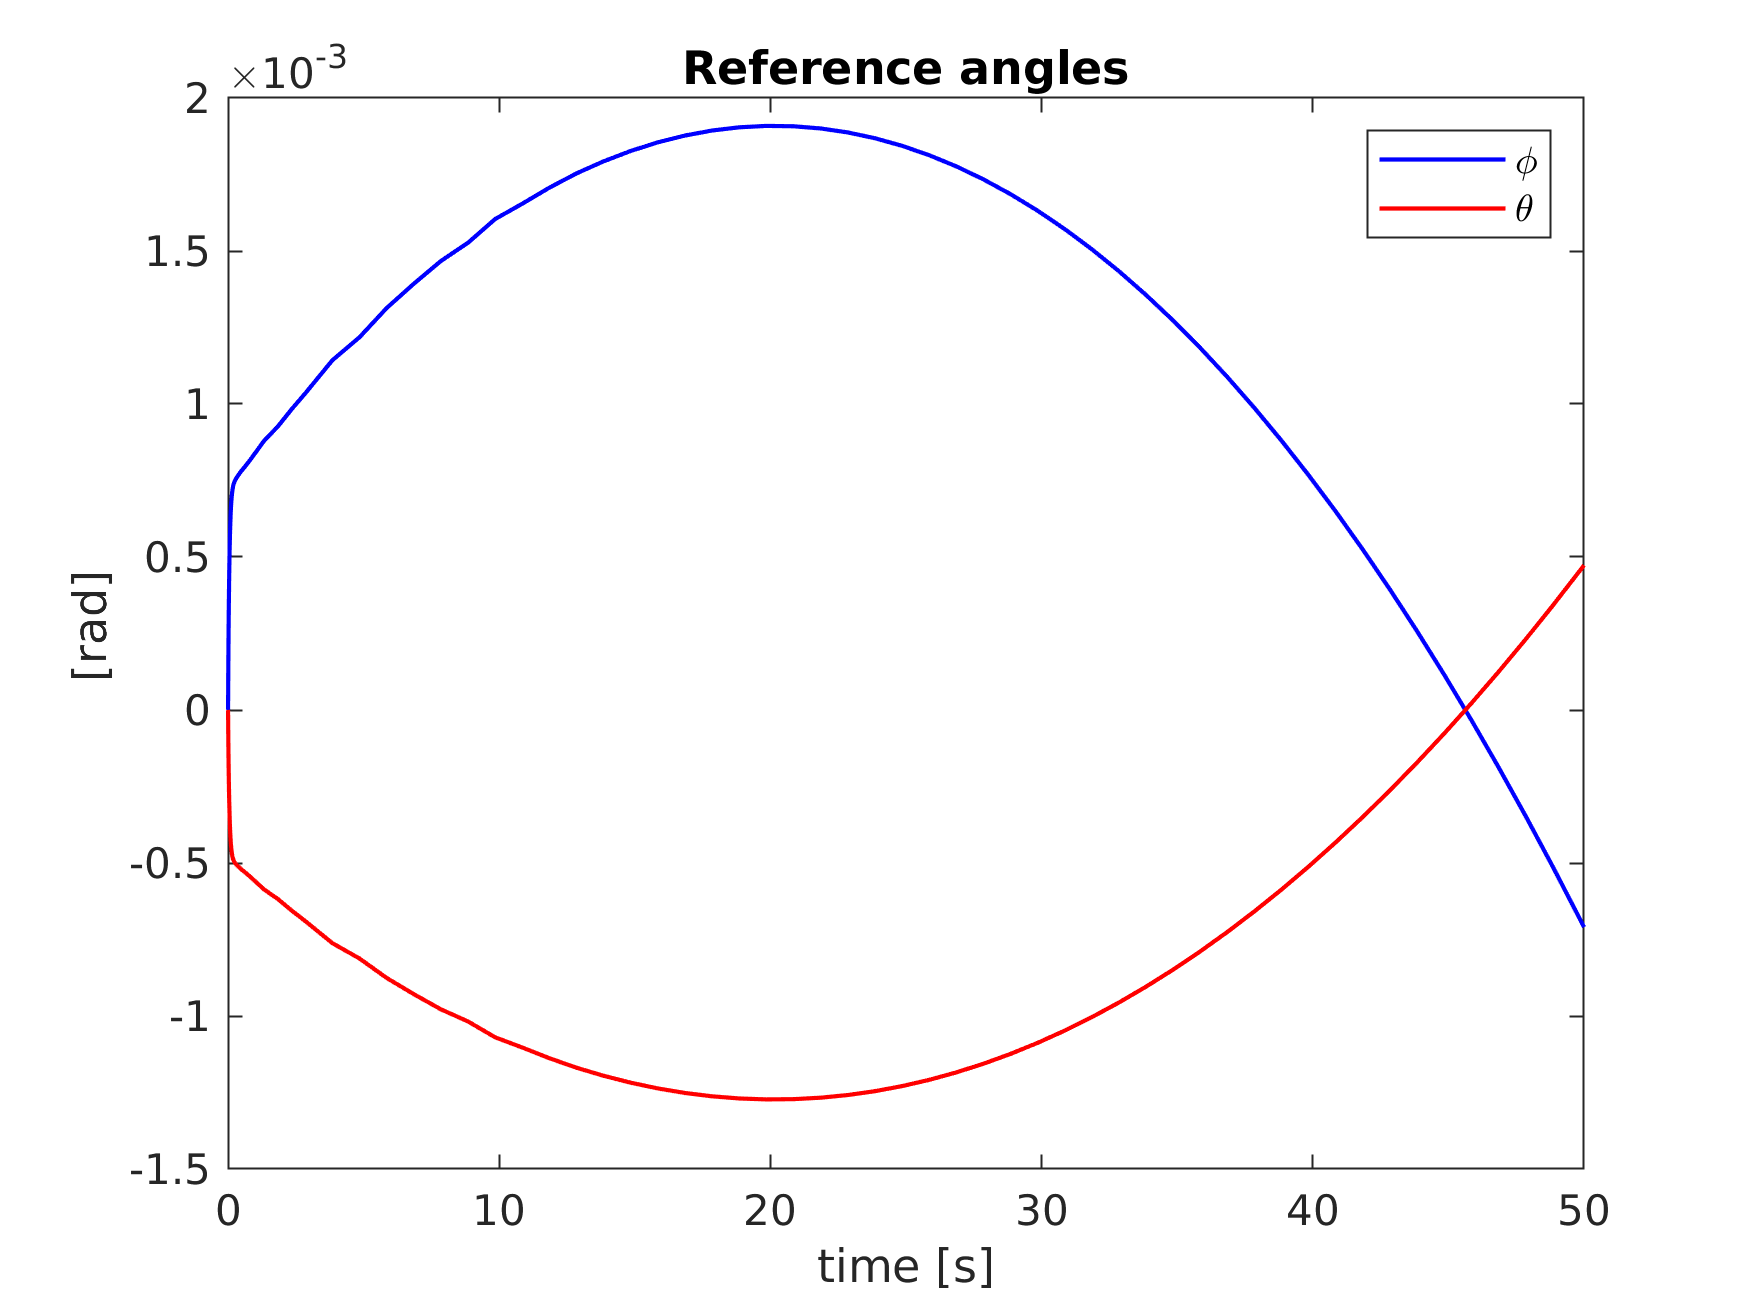
\includegraphics[width=\textwidth]{Images/AngleOuter.png}
		\caption{Reference roll and pitch angle.}
		\label{fig:outercontrolangles}
	\end{subfigure}	
	\begin{subfigure}[h!]{0.5\linewidth}
		\centering
		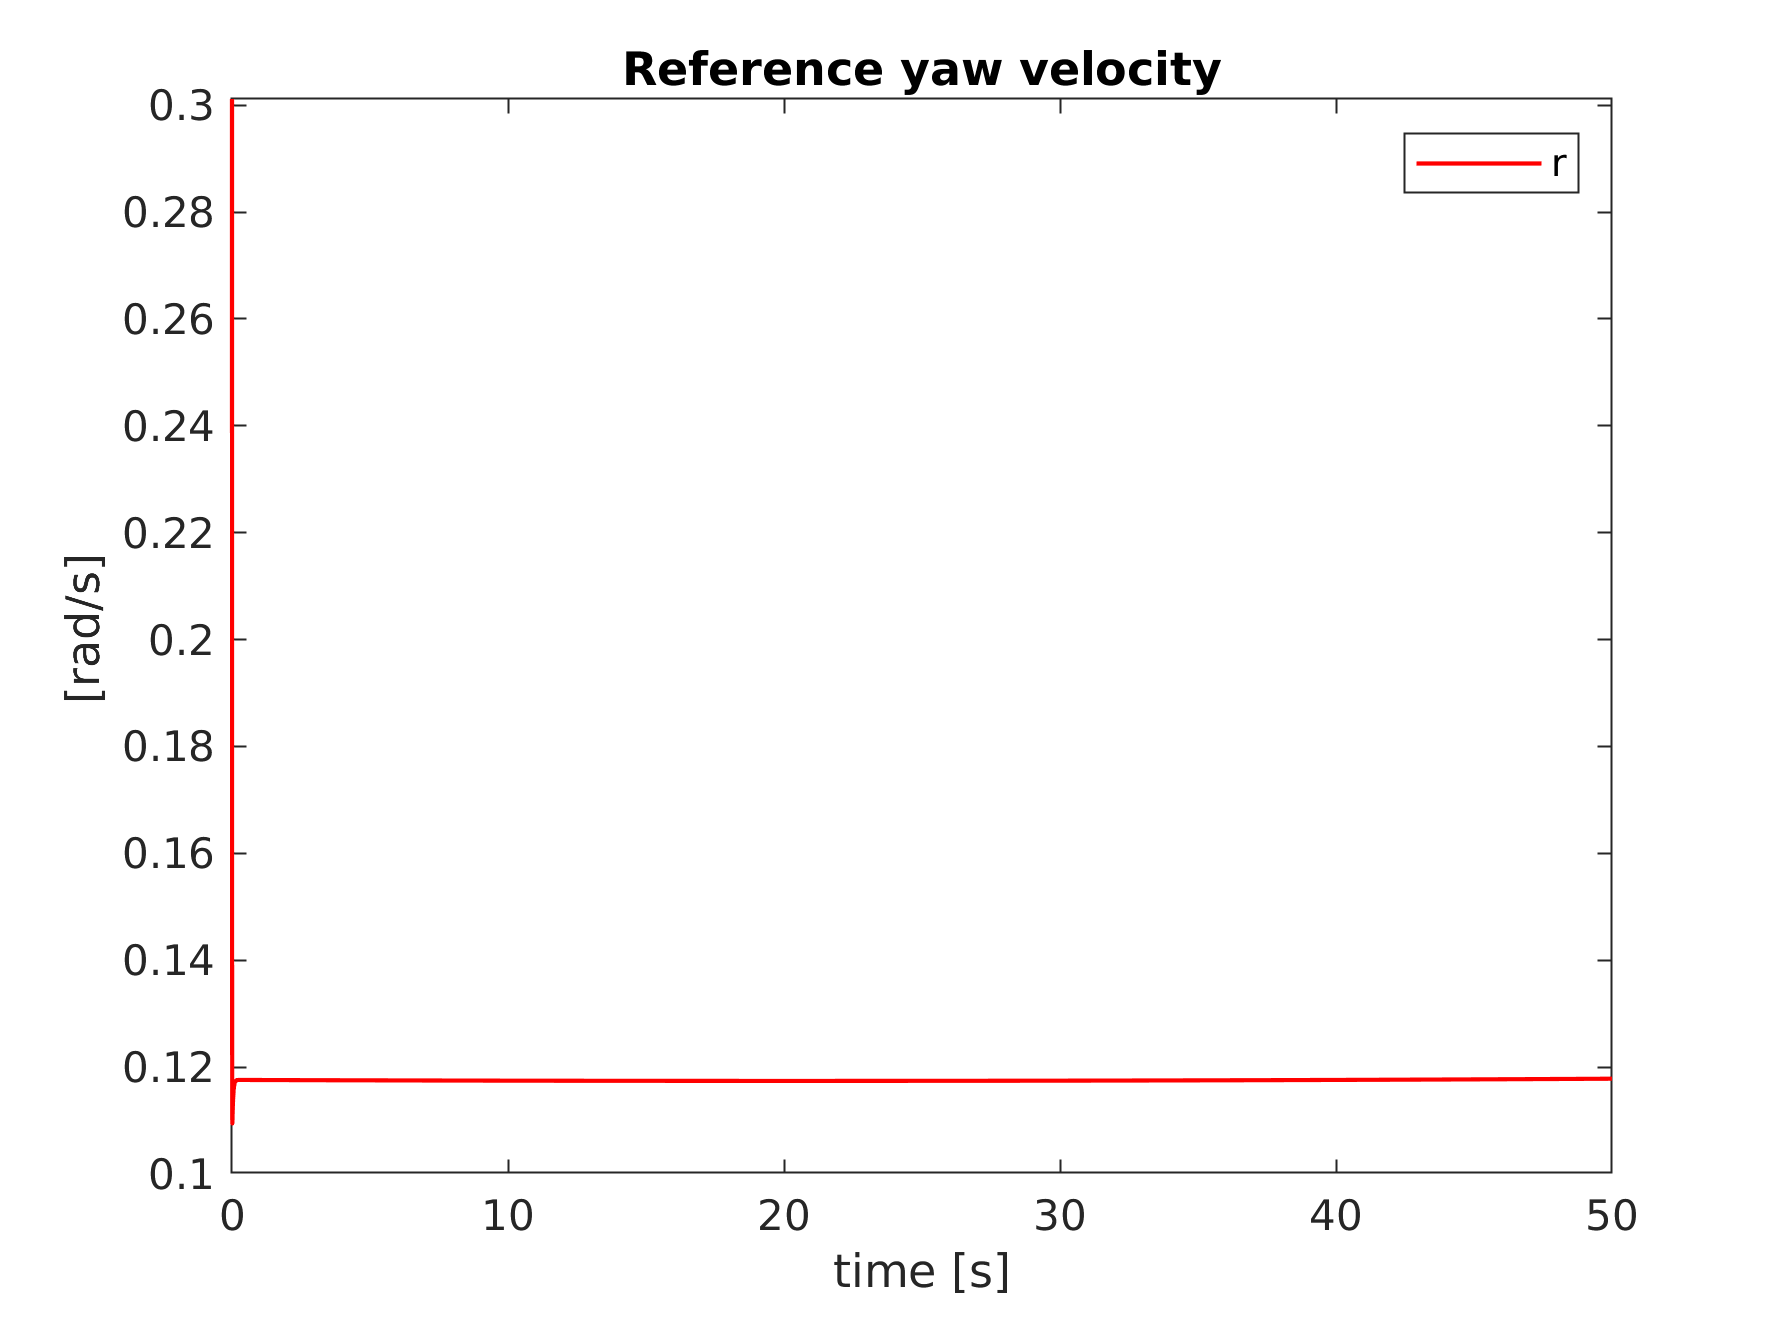
\includegraphics[width=\textwidth]{Images/velOuter.png}
		\caption{Reference yaw velocity.}
		\label{fig:outercontrolvel}
\end{subfigure}	
\caption{Reference values with cubic trajectory.}
\label{fig:ReferenceValues}
\end{figure}

For comparison we show also the plot relative to the simulation without the generation of the cubic trajectory. 

Also in this case the position is quickly regulated (fig.\ref{fig:outercontrolposNO}). However, the values coming out from the cubic trajectory generation are smoother and smaller, and hence preferable.

\begin{figure}[H]
	\centering
	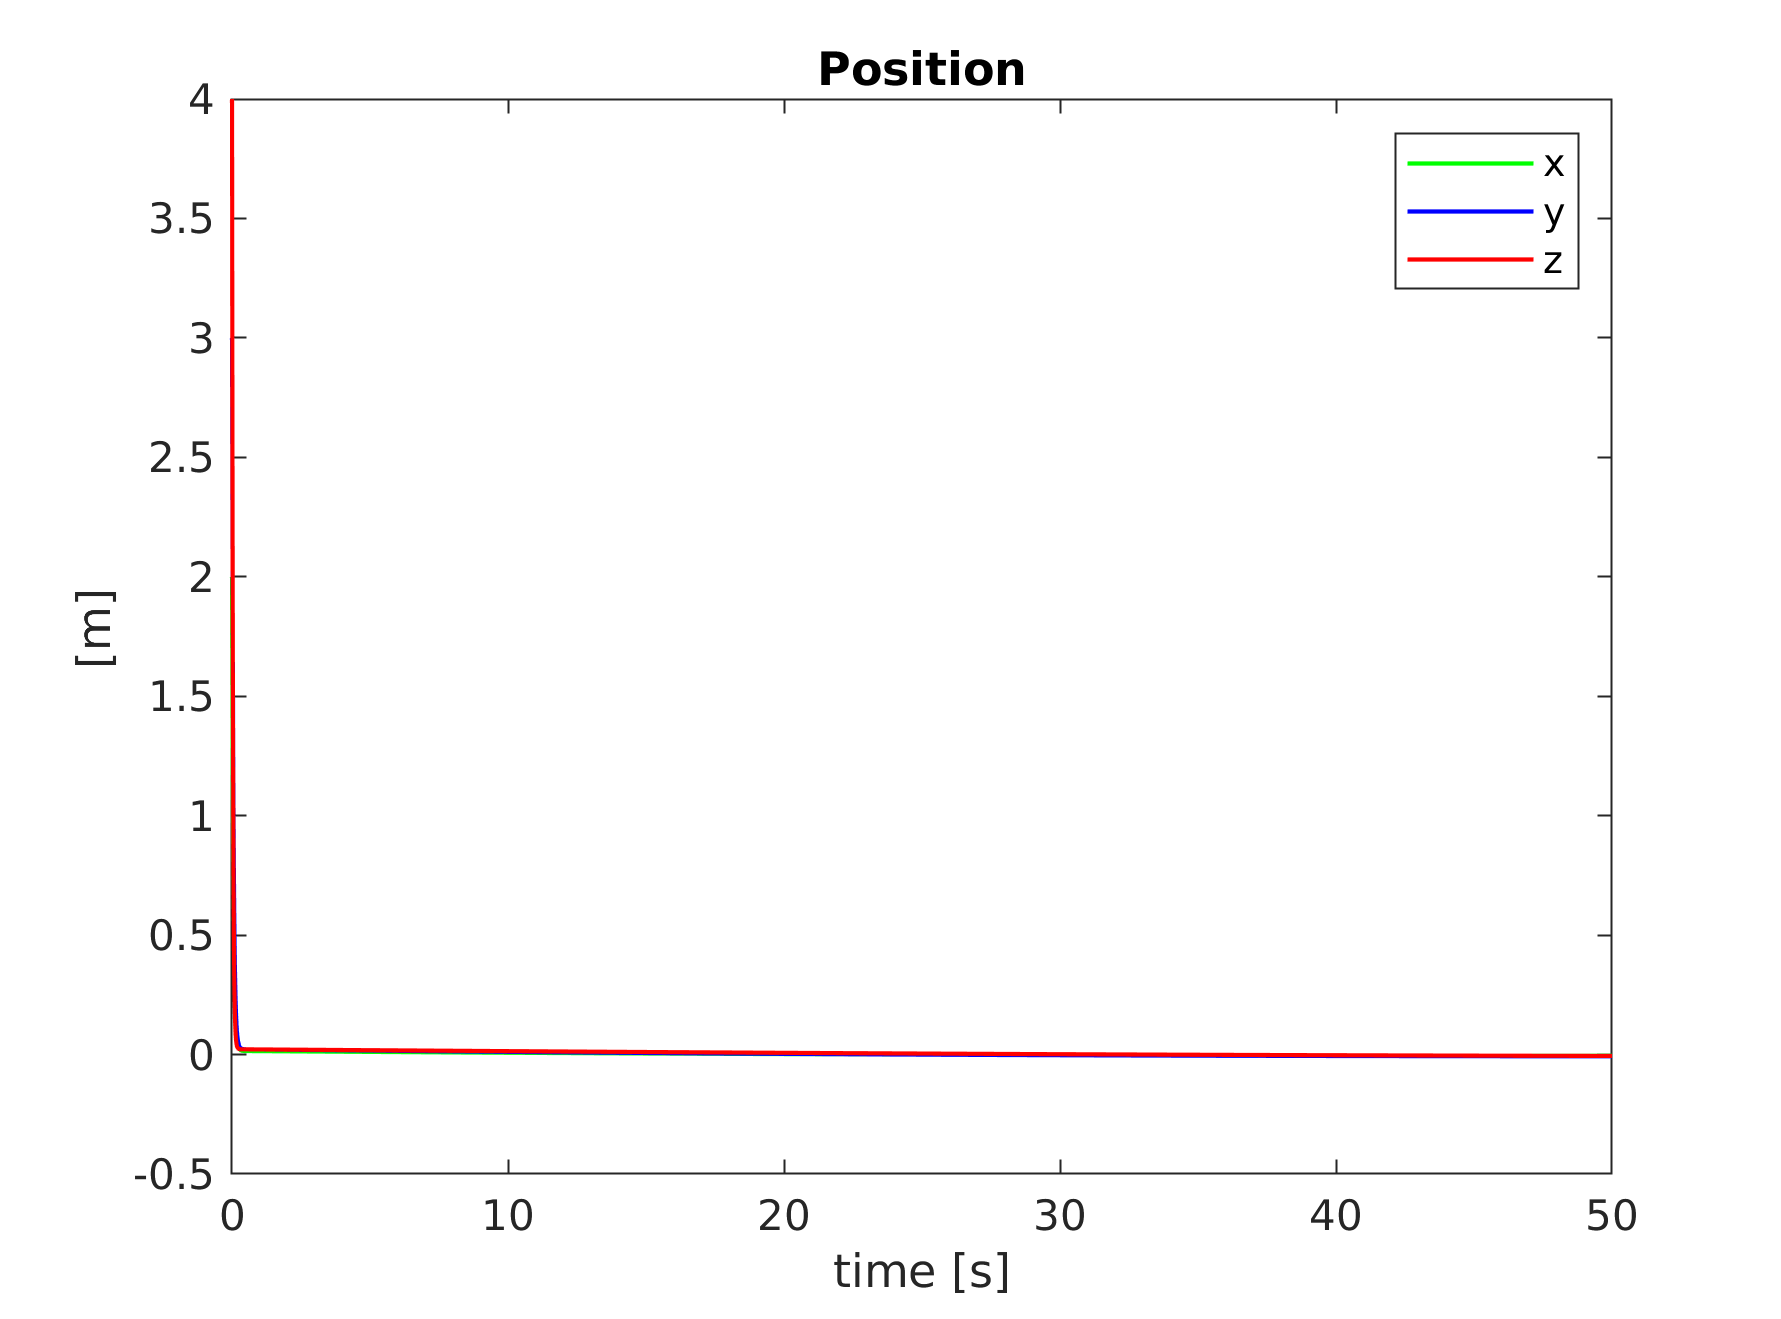
\includegraphics[width=0.7\linewidth]{Images/PositionOuterNO.png}
	\caption{Position in the Earth frame.}
	\label{fig:outercontrolposNO}	
\end{figure} 

\begin{figure}[h]
	\begin{subfigure}[h!]{0.5\linewidth}
		\centering
		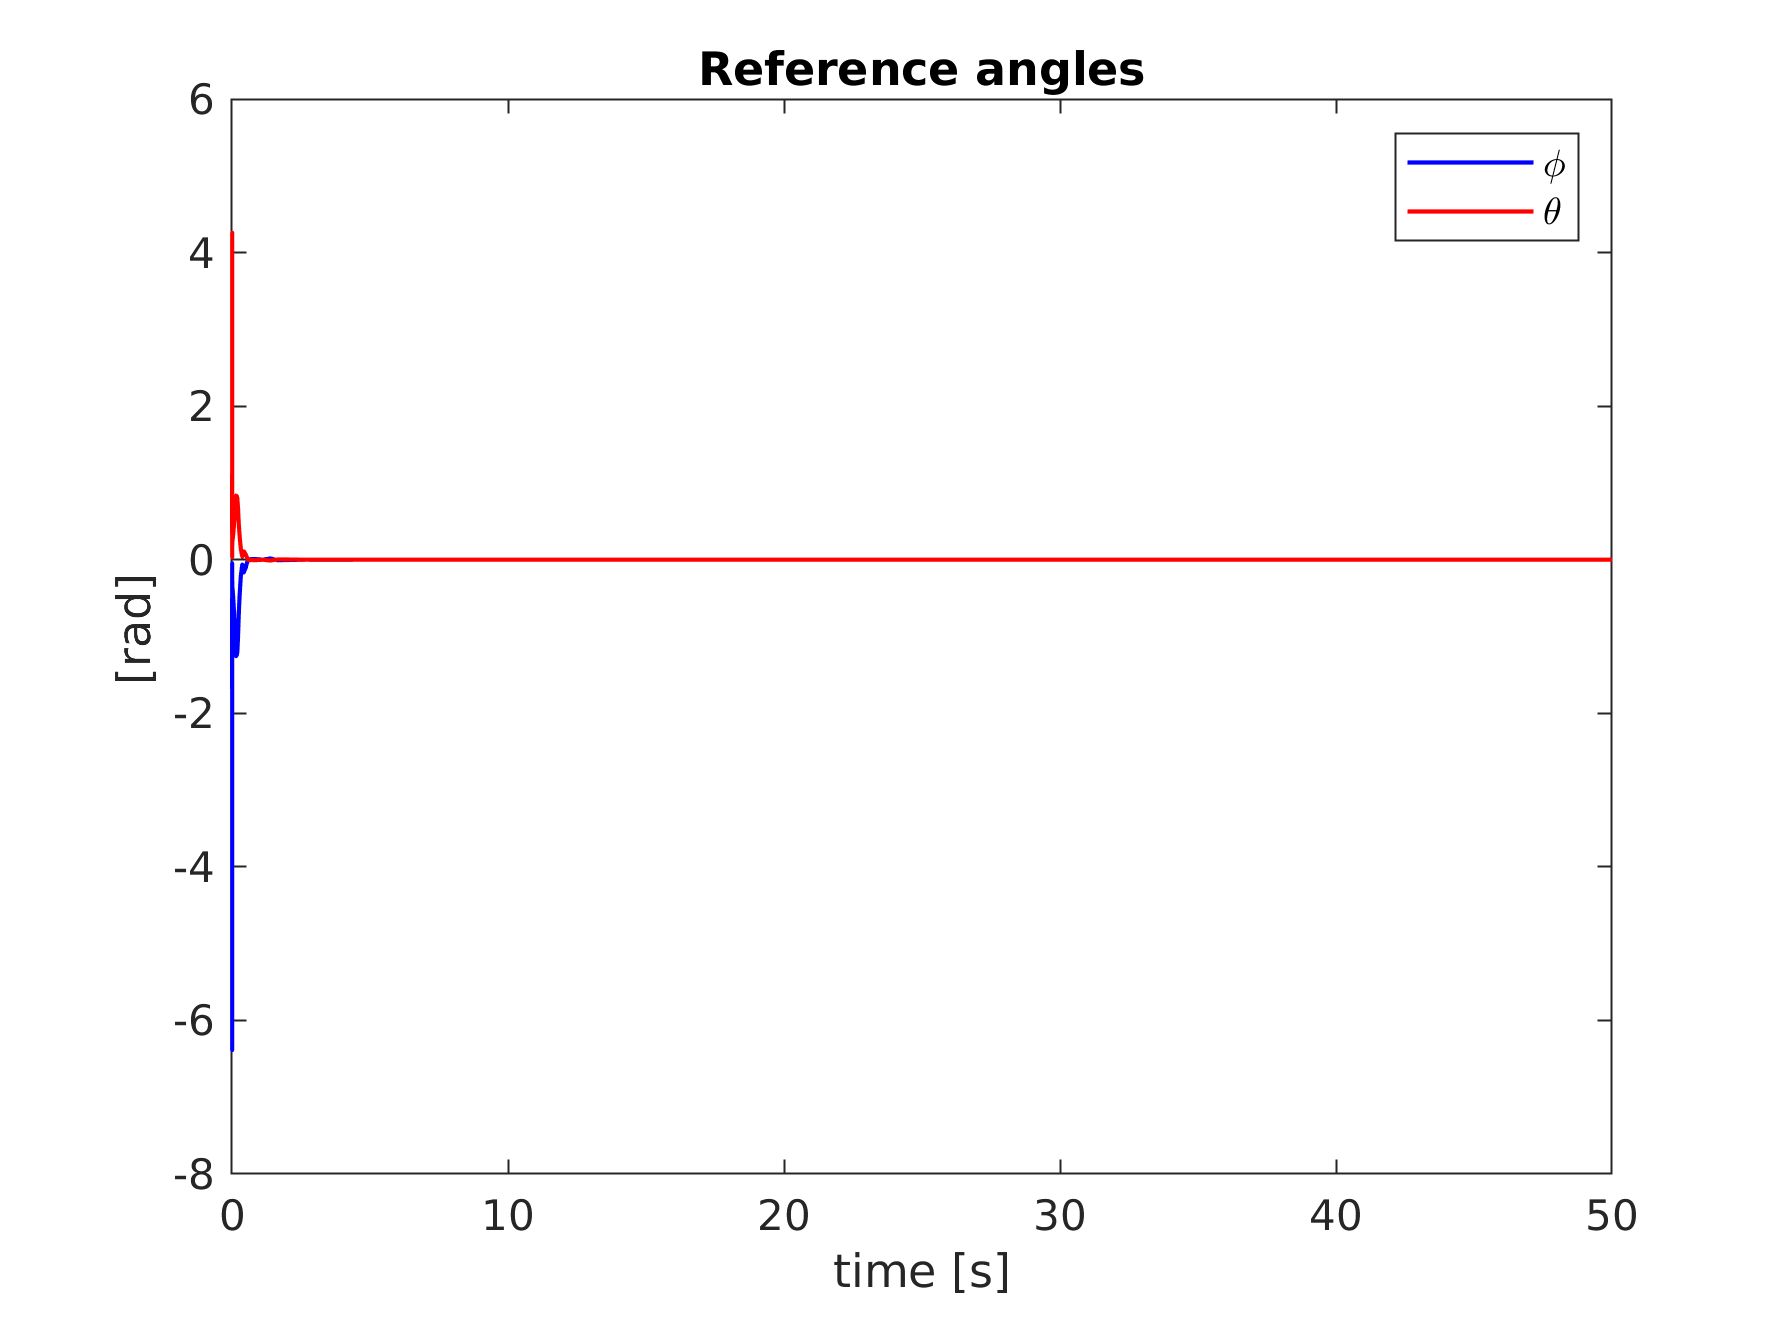
\includegraphics[width=\textwidth]{Images/AngleOuterNO.png}
		\caption{Reference roll and pitch angle.}
		\label{fig:outercontrolanglesNO}
	\end{subfigure}	
	\begin{subfigure}[h!]{0.5\linewidth}
		\centering
		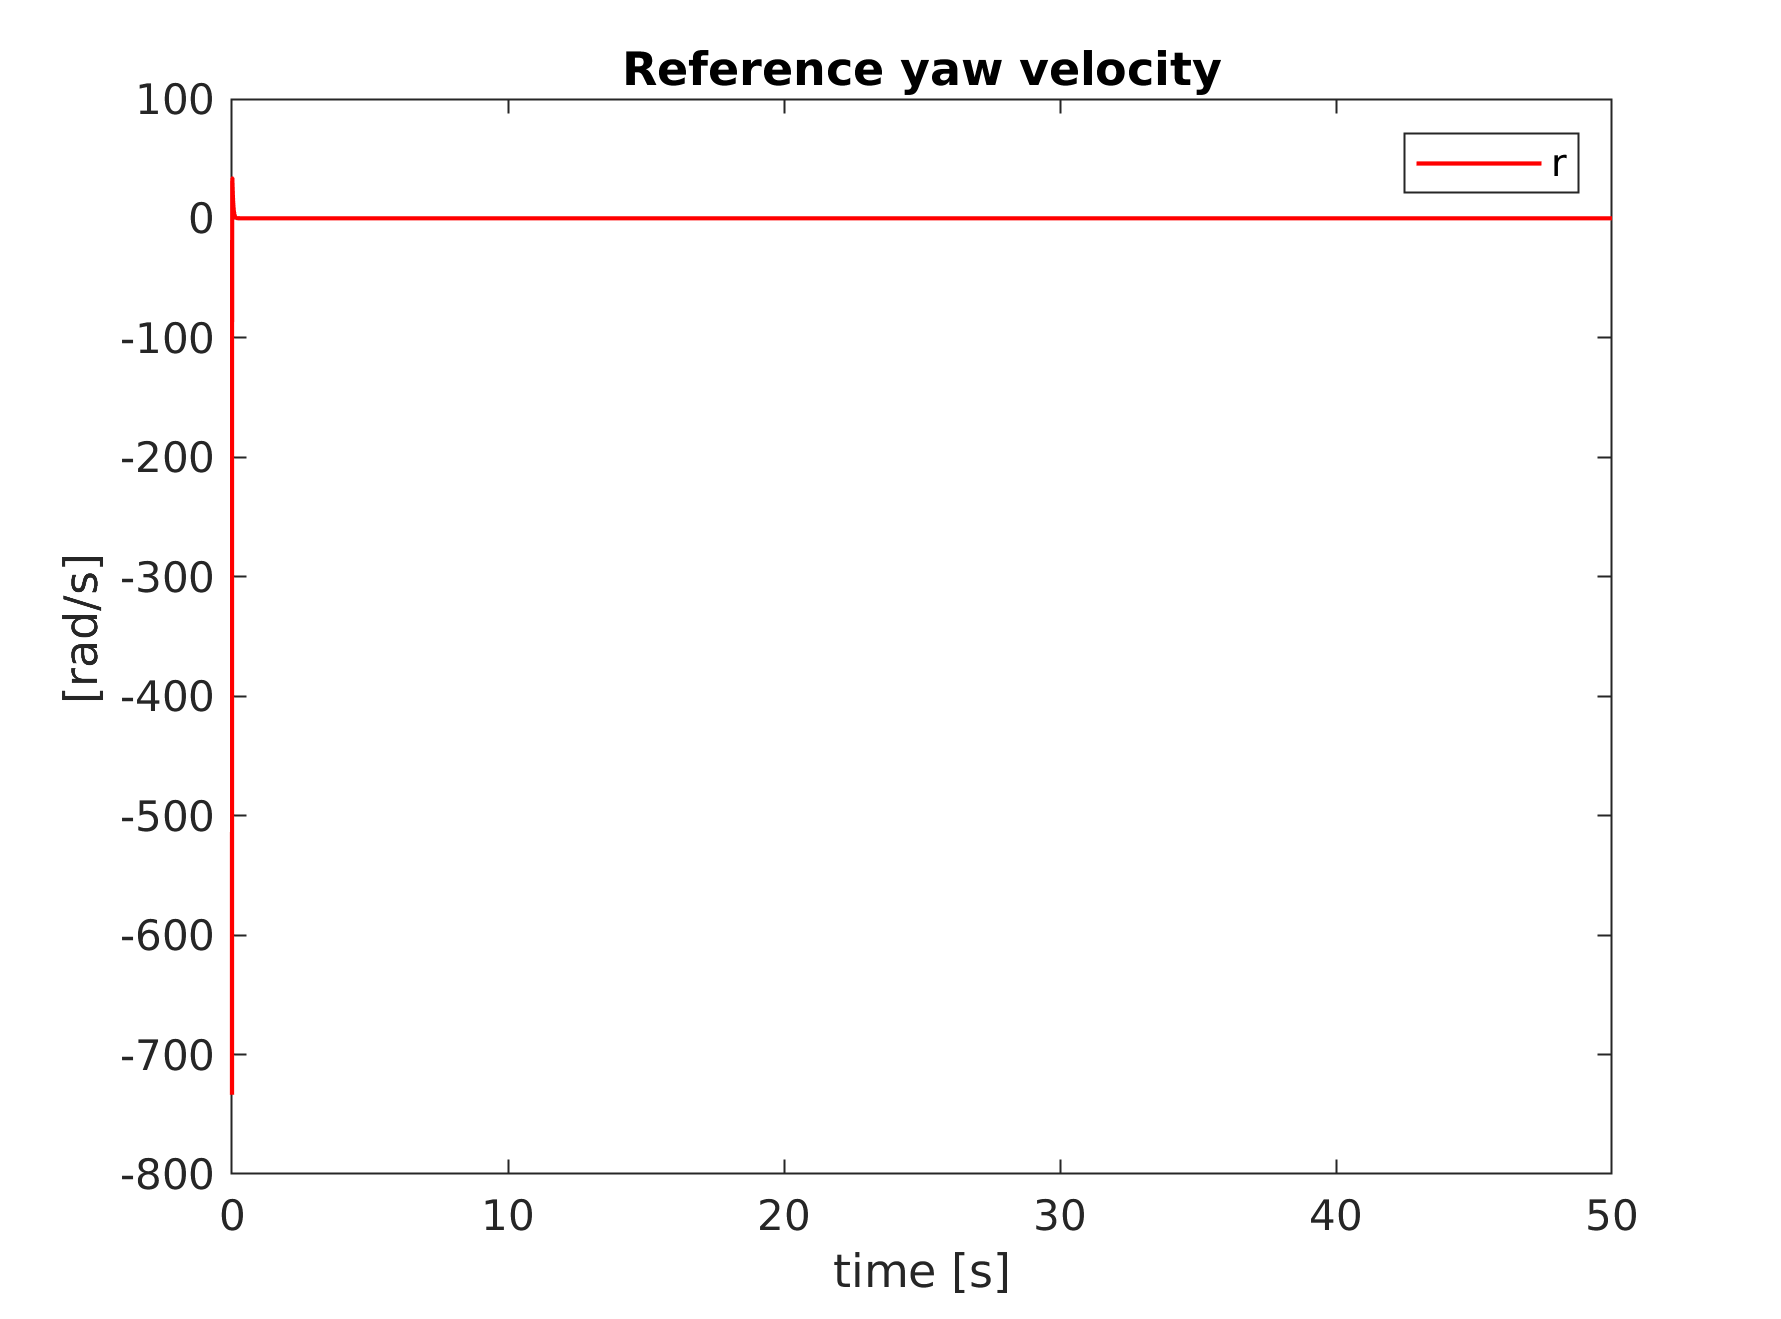
\includegraphics[width=\textwidth]{Images/velOuterNO.png}
		\caption{Reference yaw velocity.}
		\label{fig:outercontrolvelNO}
	\end{subfigure}	
\caption{Reference values with no cubic trajectory.}
\end{figure}

\subsection*{Inner control loop}

In the second simulation the task of the inner control loop is to regulate the state around a set point defined in Table \ref{FinalCondInner} from the initial condition in Table \ref{InitCondInner}.

\begin{table}
\parbox{.45\linewidth}{
	\begin{tabular}{c c c}
		\toprule
		Variable & Value & Description \\
		\midrule 
		$x_1$  & $0$ rad & $\phi$ \\
		$x_2$  & $0$ rad & $\theta$ \\
		$x_3$  & $0$ rad & $\psi$ \\
		$x_4$  & $0$ rad/s & $p$ \\
		$x_5$  & $0$ rad/s & $q$ \\
		$x_6$  & $mgd/k_r$ rad/s & $r$ \\
		\bottomrule
	\end{tabular}
	\caption{Final set point for the inner control loop simulation.}
	\label{FinalCondInner}
}
\hfill
\parbox{.45\linewidth}{	
	\begin{tabular}{c c c}
		\toprule
		Variable & Value & Description \\
		\midrule 
		$x_1$  & $-\pi/4$ rad & $\phi$ \\
		$x_2$  & $\pi/4$ rad & $\theta$ \\
		$x_3$  & $\pi/4$ rad & $\psi$ \\
		$x_4$  & $-0.5$ rad/s & $p$ \\
		$x_5$  & $0.5$ rad/s & $q$ \\
		$x_6$  & $2.7$ rad/s & $r$ \\
		\bottomrule
	\end{tabular}
	\caption{Initial conditions for the inner control loop simulation.}
	\label{InitCondInner}
}
\end{table}

The simulation time is $ 5 $ seconds. As shown in fig.\ref{fig:innercontrolvel} and fig.\ref{fig:innercontrolangles} the values of both angles and velocities are perfectly regulated. In particular the spinning velocity converges to the value $ \frac{mgd}{k_r} $, relative to the hovering condition.

\begin{figure}[H]
	\centering
	\begin{subfigure}[h!]{0.7\linewidth}
	\centering
	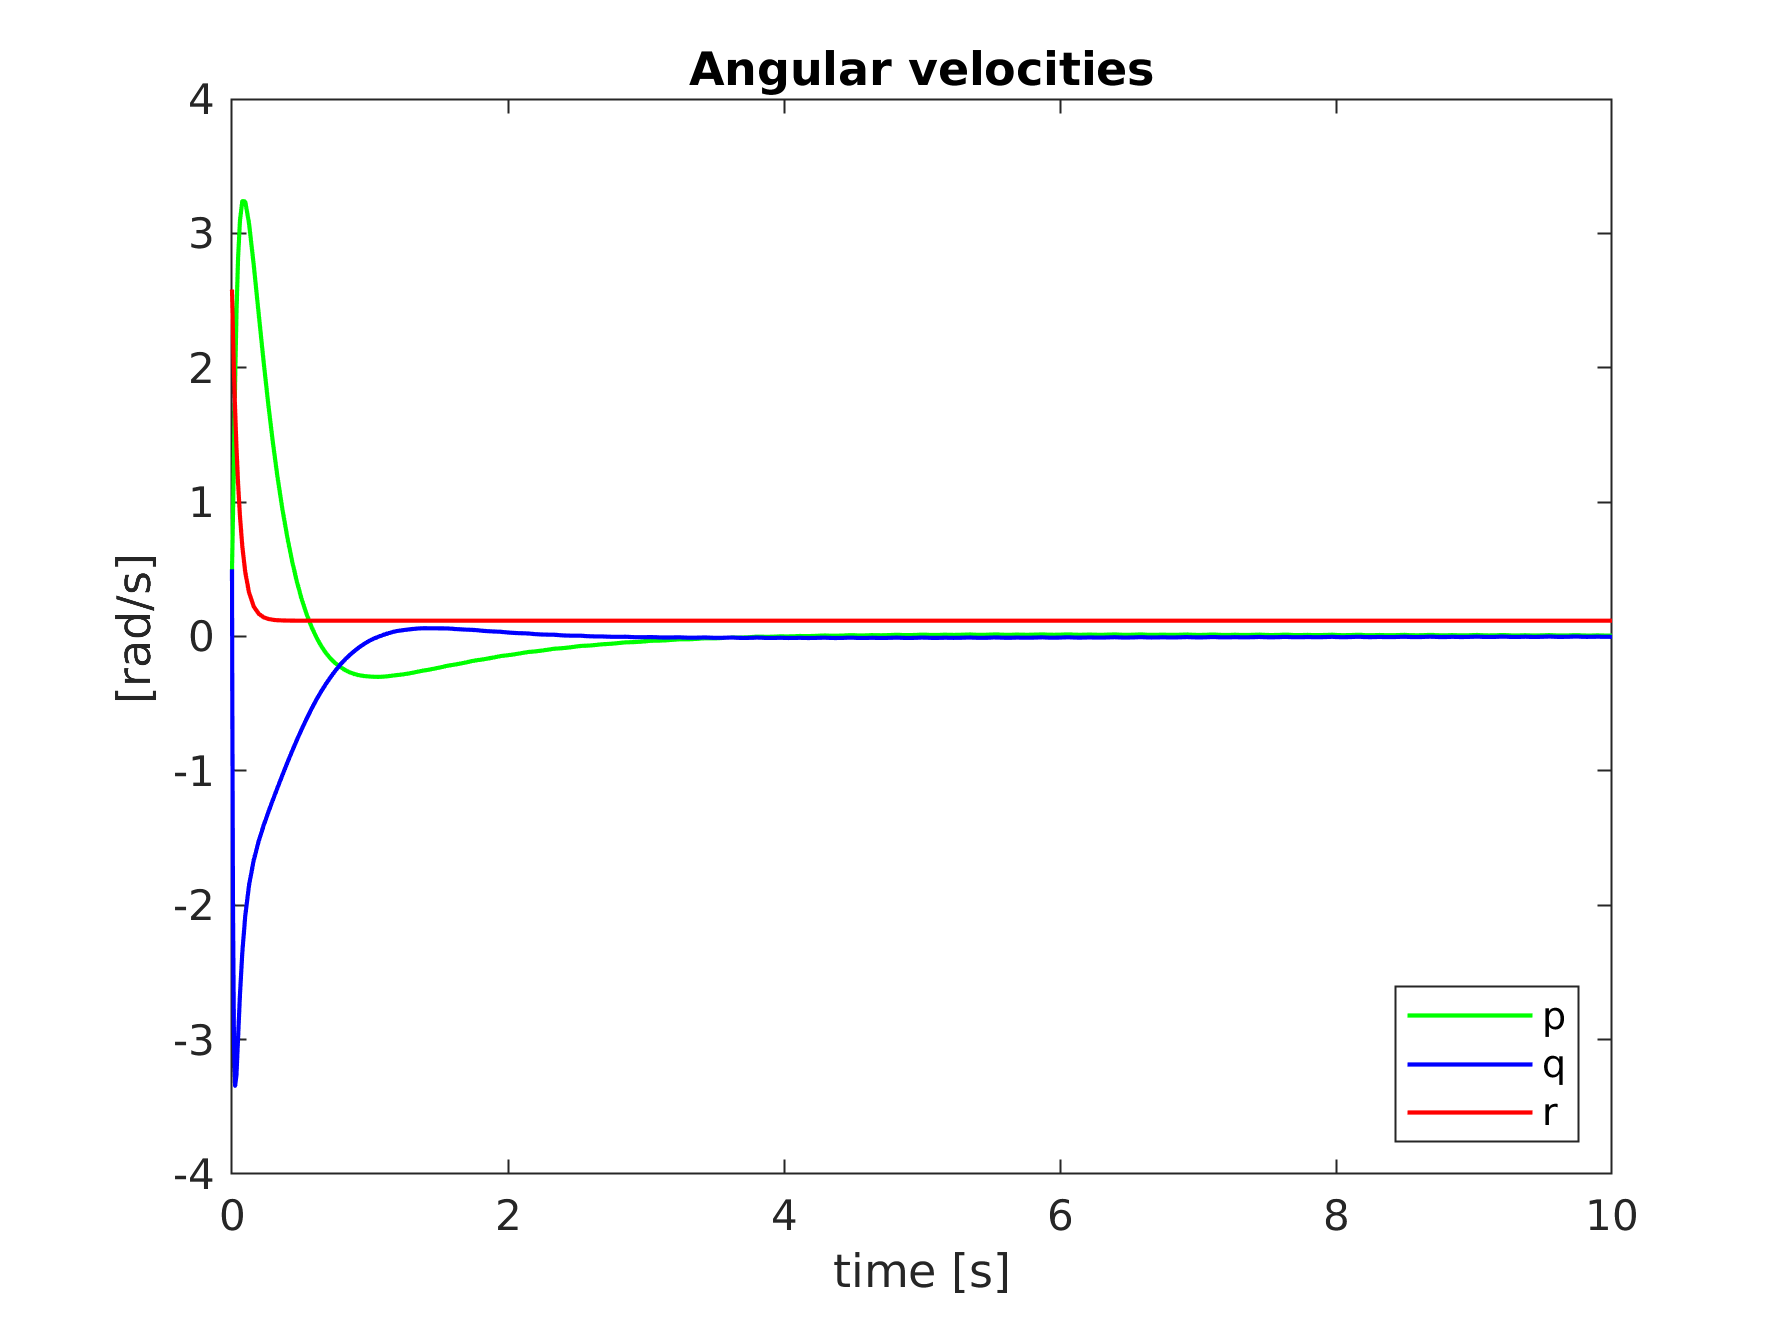
\includegraphics[width=\textwidth]{Images/innerControlVel}
	\caption{}
	\label{fig:innercontrolvel}	
	\end{subfigure} \hfill
	\begin{subfigure}[h!]{0.7\linewidth}
	\centering
	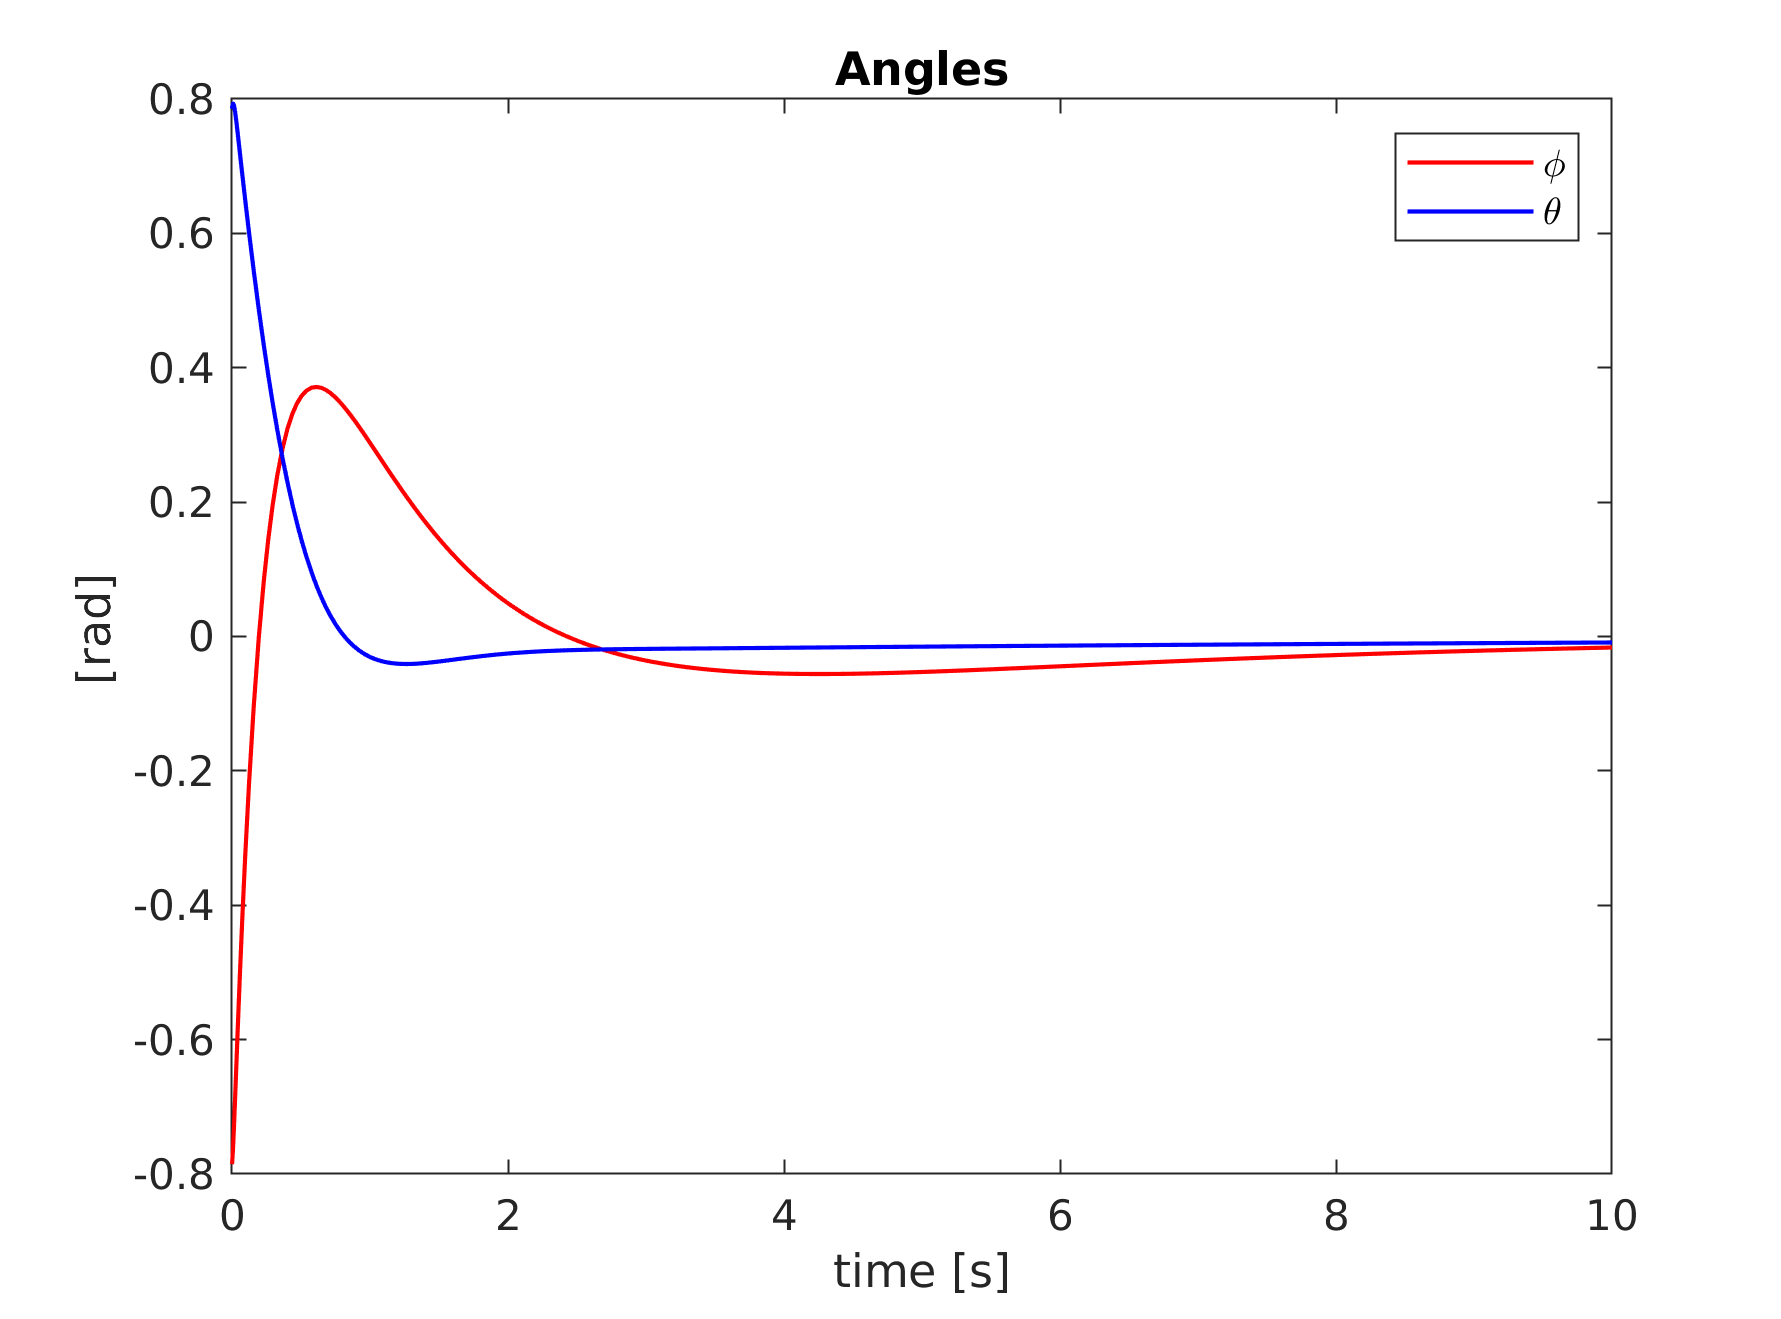
\includegraphics[width=\textwidth]{Images/innerControlAngles}
	\caption{}
	\label{fig:innercontrolangles}
	\end{subfigure}	
	\caption{Values of angles and velocities relative to the inner control loop.}
\end{figure}

The rotor forces, after an initial peak due to the pretty large error, remains constant and assume small values (fig.\ref{fig:forcesiInner}). In particular $ f_1 $ and $ f_3 $ are used to sustain the vehicle in hovering flight and $ f_4 $ deals with the regulation of spinning velocity.

\begin{figure}
	\centering
	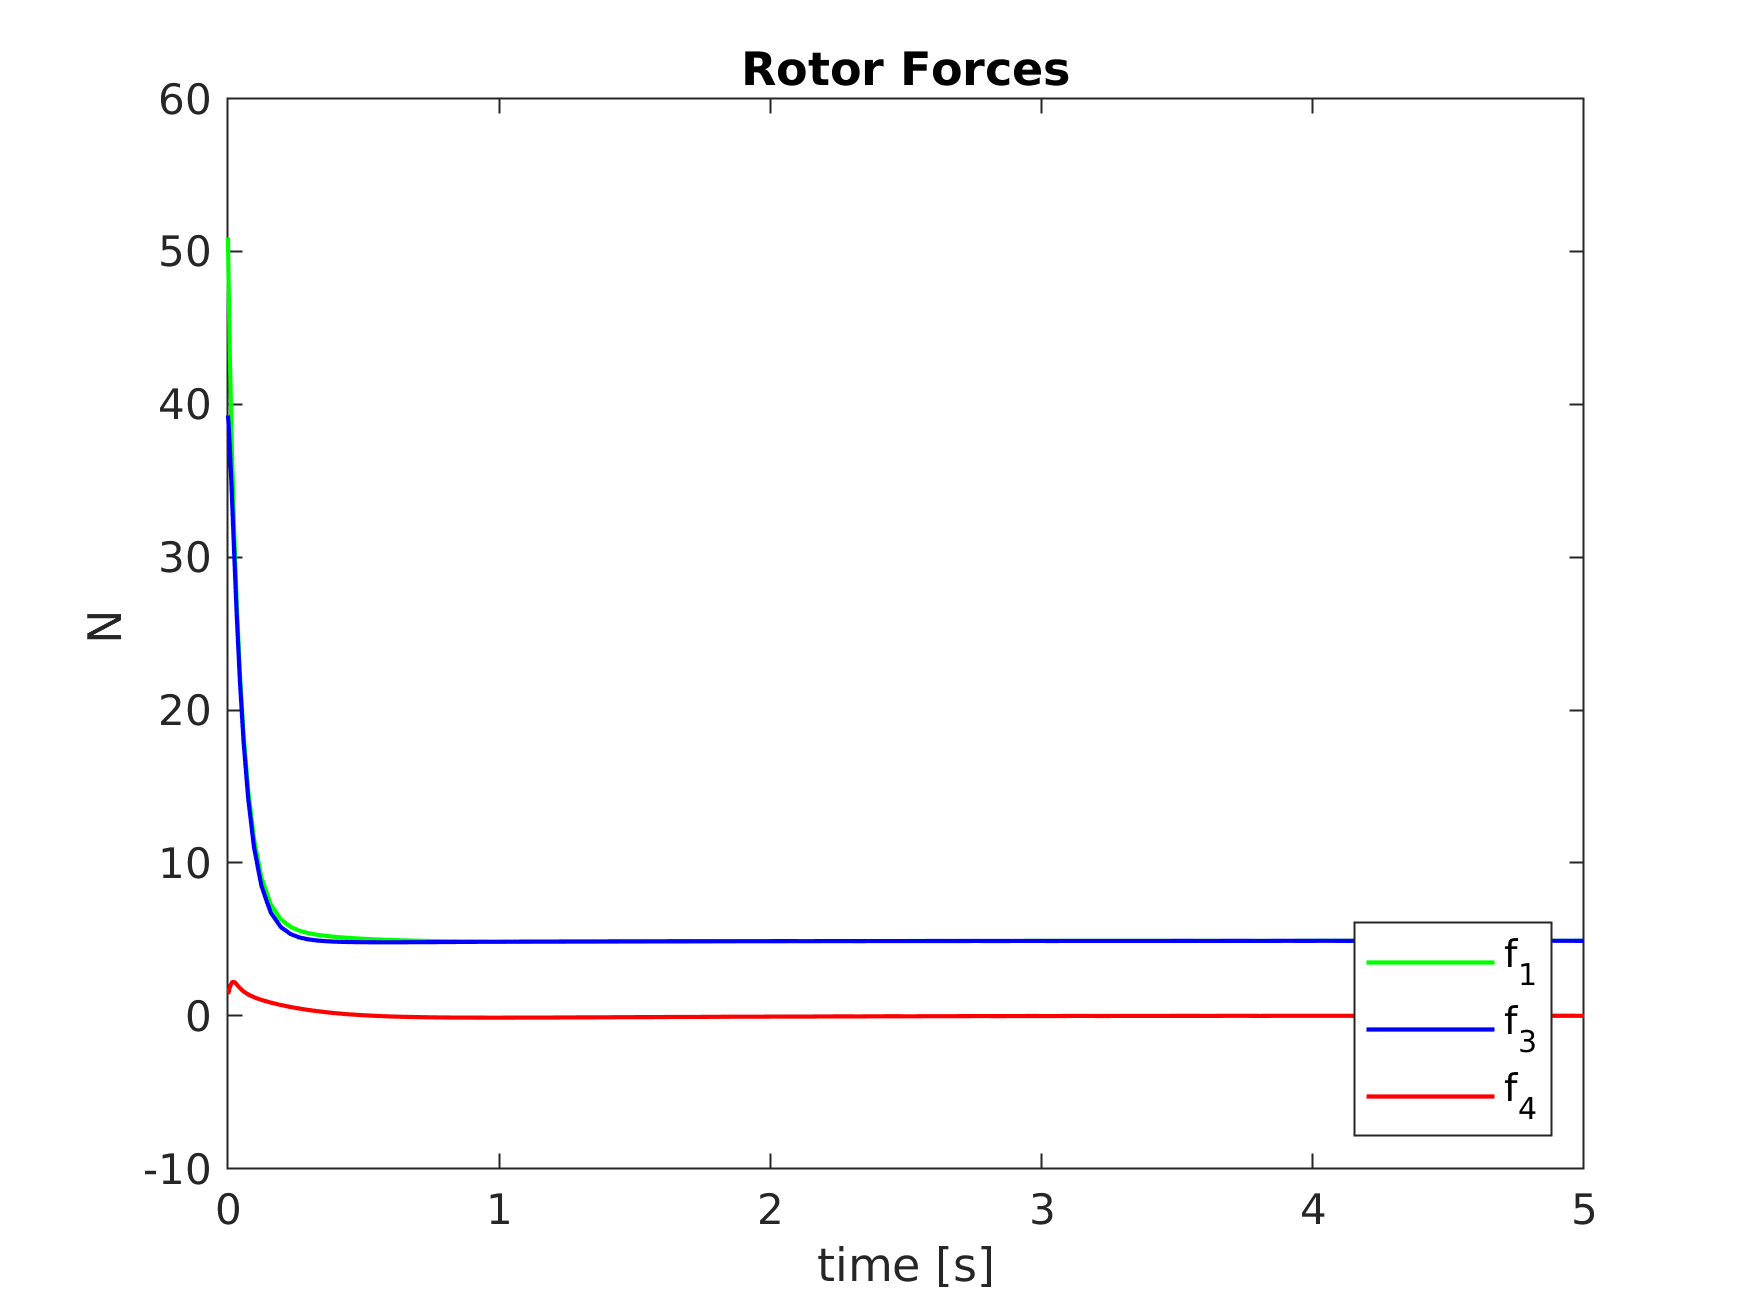
\includegraphics[width=0.7\linewidth]{Images/ForcesInner}
	\caption{Forces computed from the inputs of the inner control loop.}
	\label{fig:forcesiInner}
\end{figure}

\section*{Complete simulation}

In the simulations of this section, both the outer and the inner control loop are activated. 

The simulation time is 100 seconds. The controller must fly the quadrotor from the initial condition in Table \ref{SimulationInit} to the origin of the Earth frame. 

\begin{table}
	\centering
	\begin{tabular}{c c c}
		\toprule
		Variable & Value & Description \\
		\midrule 
		$x_1$  & $0.1$ rad & $\phi$ \\
		$x_2$  & $-0.1$ rad & $\theta$ \\
		$x_3$  & $0.1$ rad & $\psi$ \\
		$x_4$  & $0.2$ rad/s & $p$ \\
		$x_5$  & $-0.2$ rad/s & $q$ \\
		$x_6$  & $0.15$ rad/s & $r$ \\
		$x_7$  & $5$ m & $x$ \\
		$x_8$  & $5$ m & $y$ \\
		$x_9$  & $5$ m & $z$ \\
		$x_{10}$  & $0$ m/s & $\dot{x}$ \\
		$x_{11}$  & $0$ m/s & $\dot{y}$ \\
		$x_{12}$  & $0$ m/s & $\dot{z}$ \\
		\bottomrule
	\end{tabular}
	\caption{Initial conditions for the complete simulation.}
	\label{SimulationInit}
\end{table}


As shown in fig.\ref{fig:position}, the vertical trajectory of the vehicle is perfectly tracked (red line). Instead, the horizontal position (green and blue lines) oscillates around the planned trajectory: the outer loop control has small gains so as to be slow enough. It correct the error not aggressively, generating reference angles that do not change quickly.

The inner control loop regulates successfully the reference angles. In fig.\ref{fig:angles_error} it is clear how the error between the desired and the actual roll and pitch angles is suddenly reduced to zero.

Also in this case the forces, after an initial peak, become constant. In particular $ \mathcal{M}_1 $ and $ \mathcal{M}_3 $ rotors sustain the vehicle. The rotor $ \mathcal{M}_4 $ provides a periodical thrust (fig.\ref{fig:r4force} - zoom-in): the outer controller generates a time varying references for the inner control loop that depends one the rotation matrix in eq.\eqref{rotation_matrix_outer} in order to achieve the desired horizontal translation. To this effect, the rotor $ \mathcal{M}_4 $ tries to regulate the direction of the total thrust, allowing the translation. 

\begin{figure}[H]
	\centering
	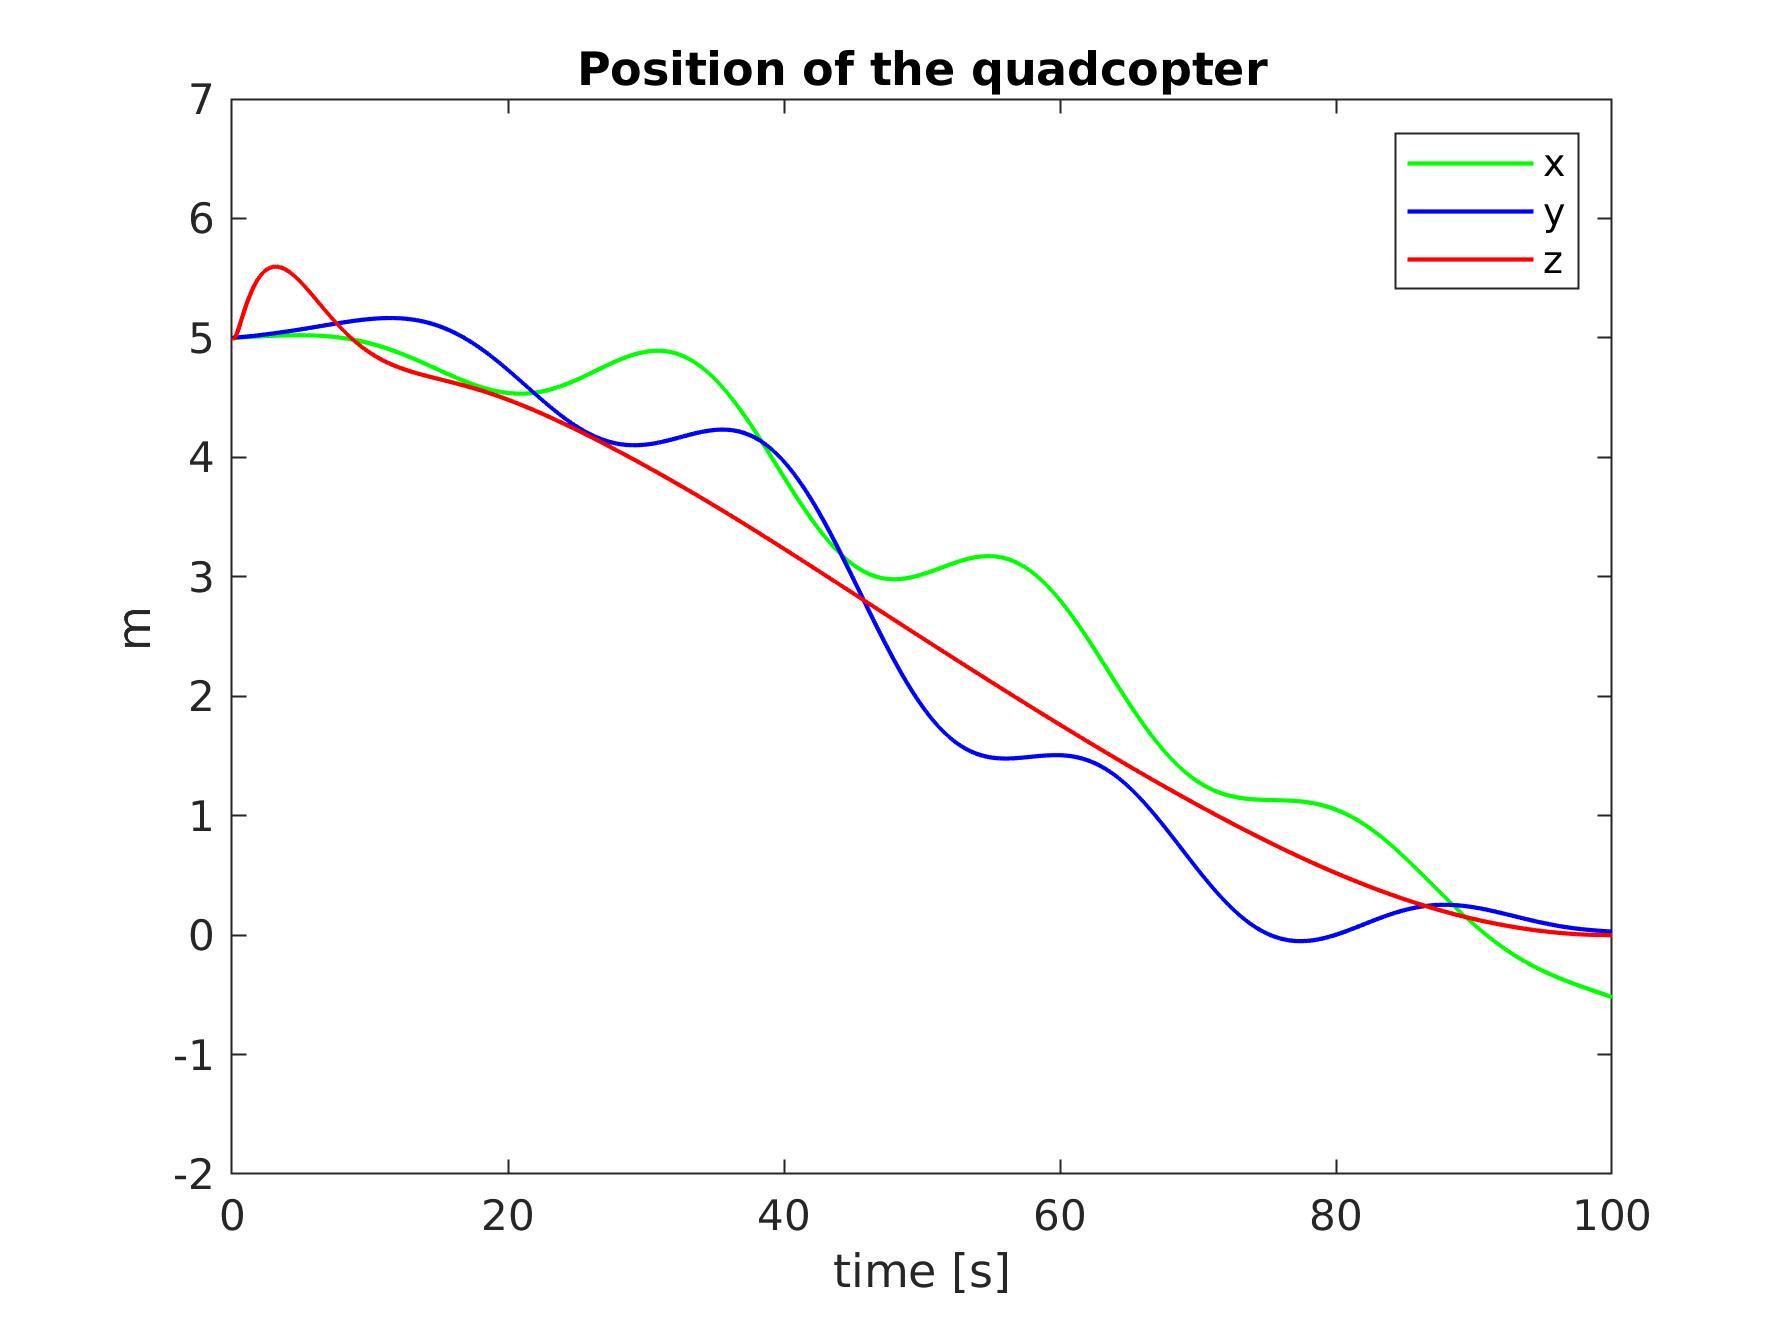
\includegraphics[width=0.7\linewidth]{Images/Position}
	\caption{Position of the quadcopter in the Earth frame.}
	\label{fig:position}
\end{figure}

\begin{figure}
	\centering
	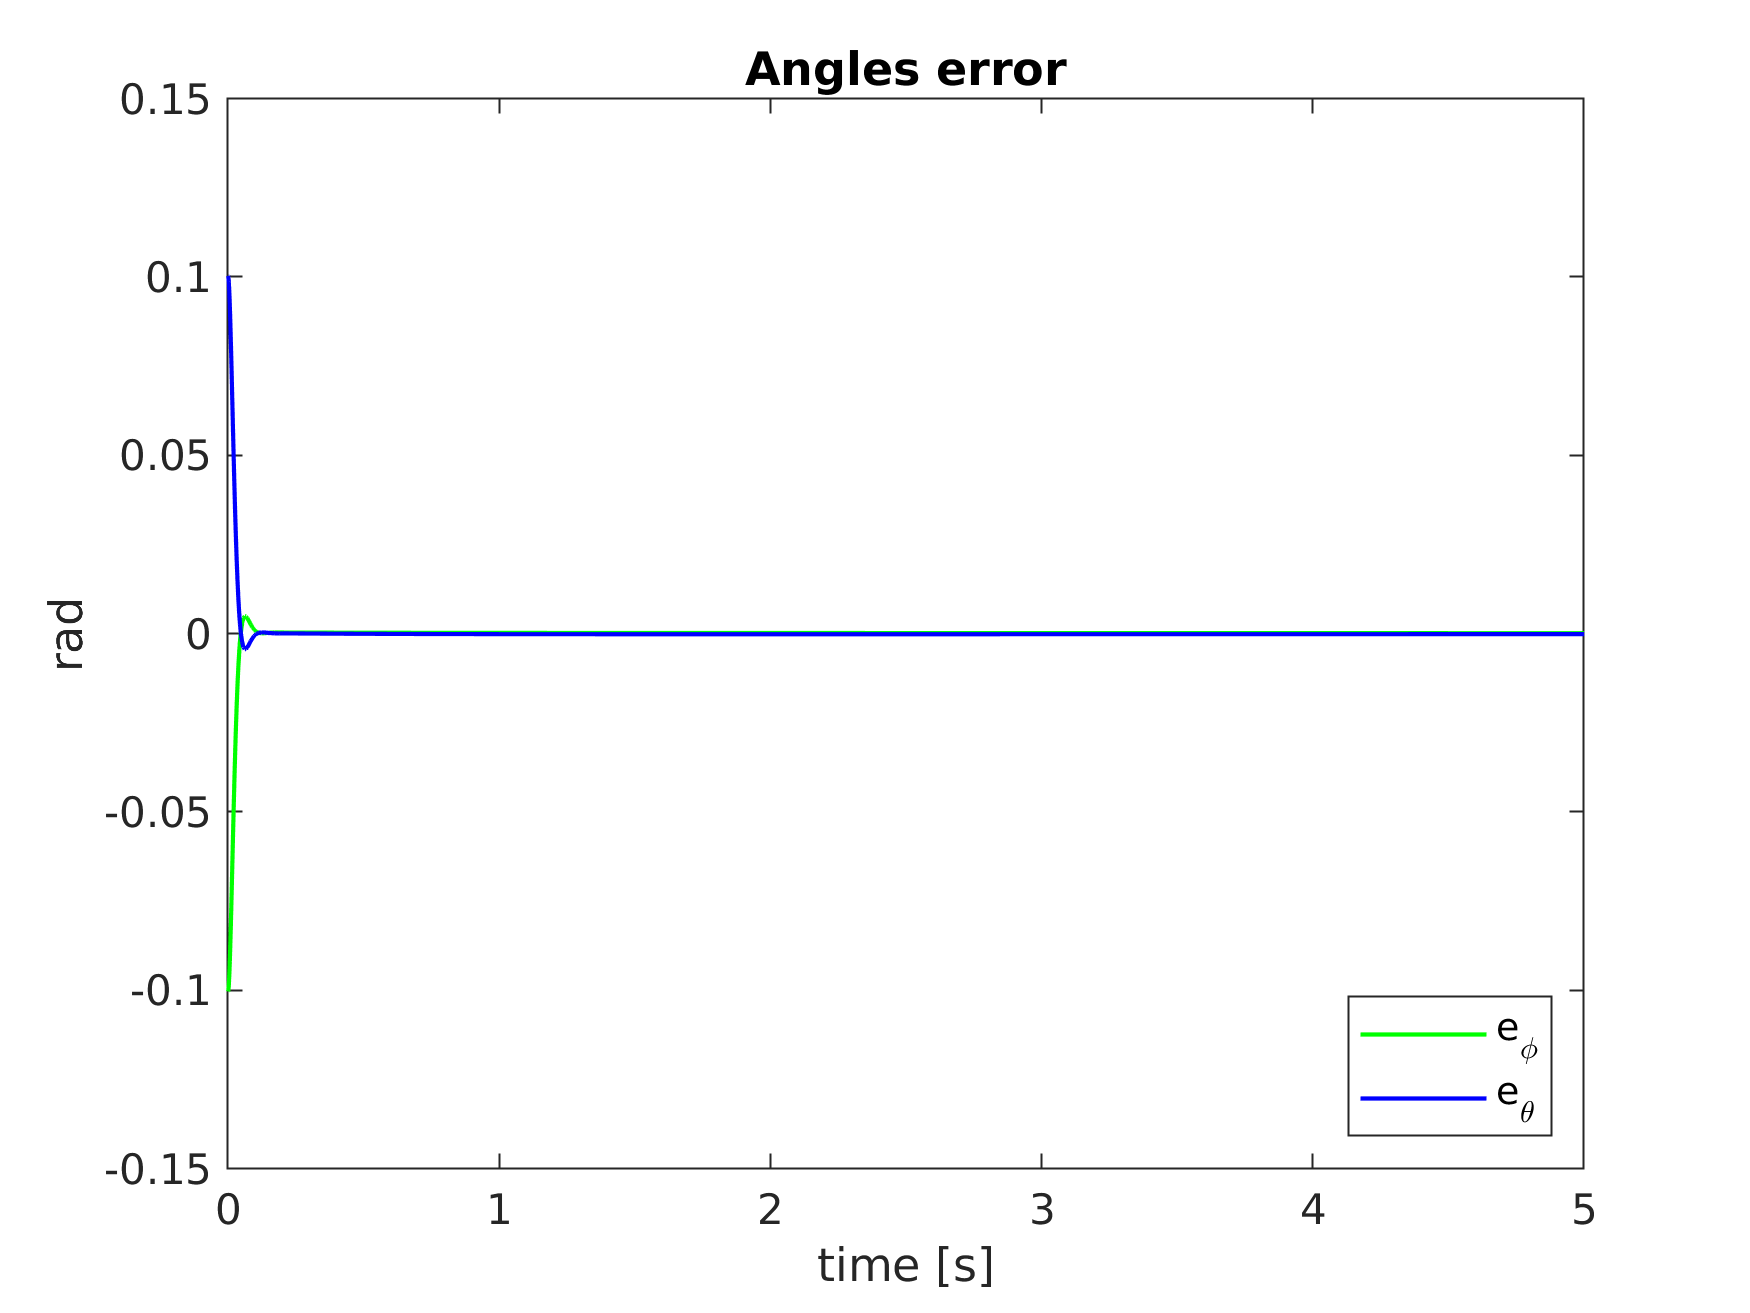
\includegraphics[width=0.7\linewidth]{Images/Angles_error}
	\caption{Error between the desired and the actual roll and pitch angles - only the first 5 seconds.}
	\label{fig:angles_error}
\end{figure}

\begin{figure}
	\centering
	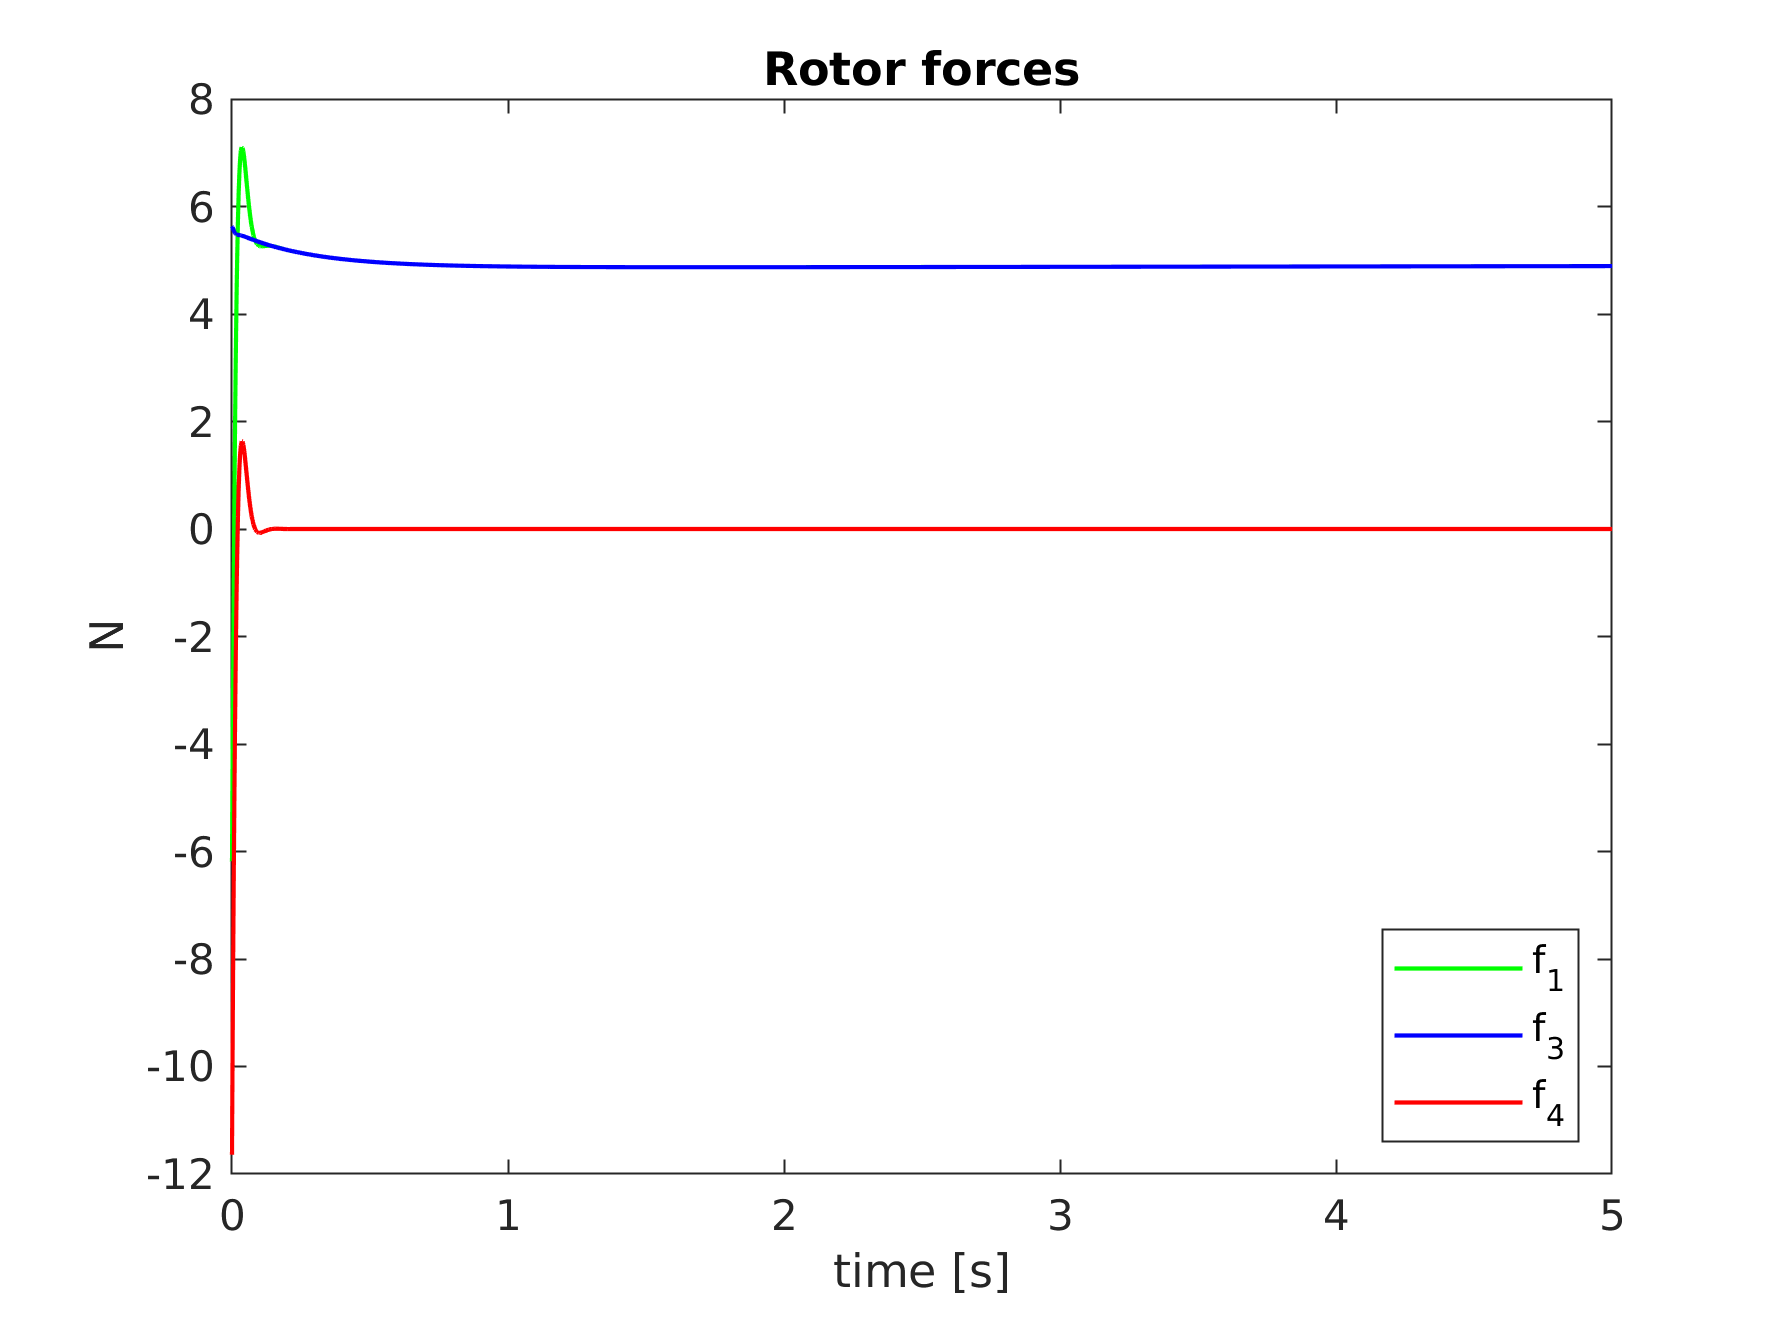
\includegraphics[width=0.7\linewidth]{Images/Forces}
	\caption{Forces required by the double-loop controller - only the first 5 seconds.}
	\label{fig:forces}
\end{figure}

\begin{figure}
	\centering
	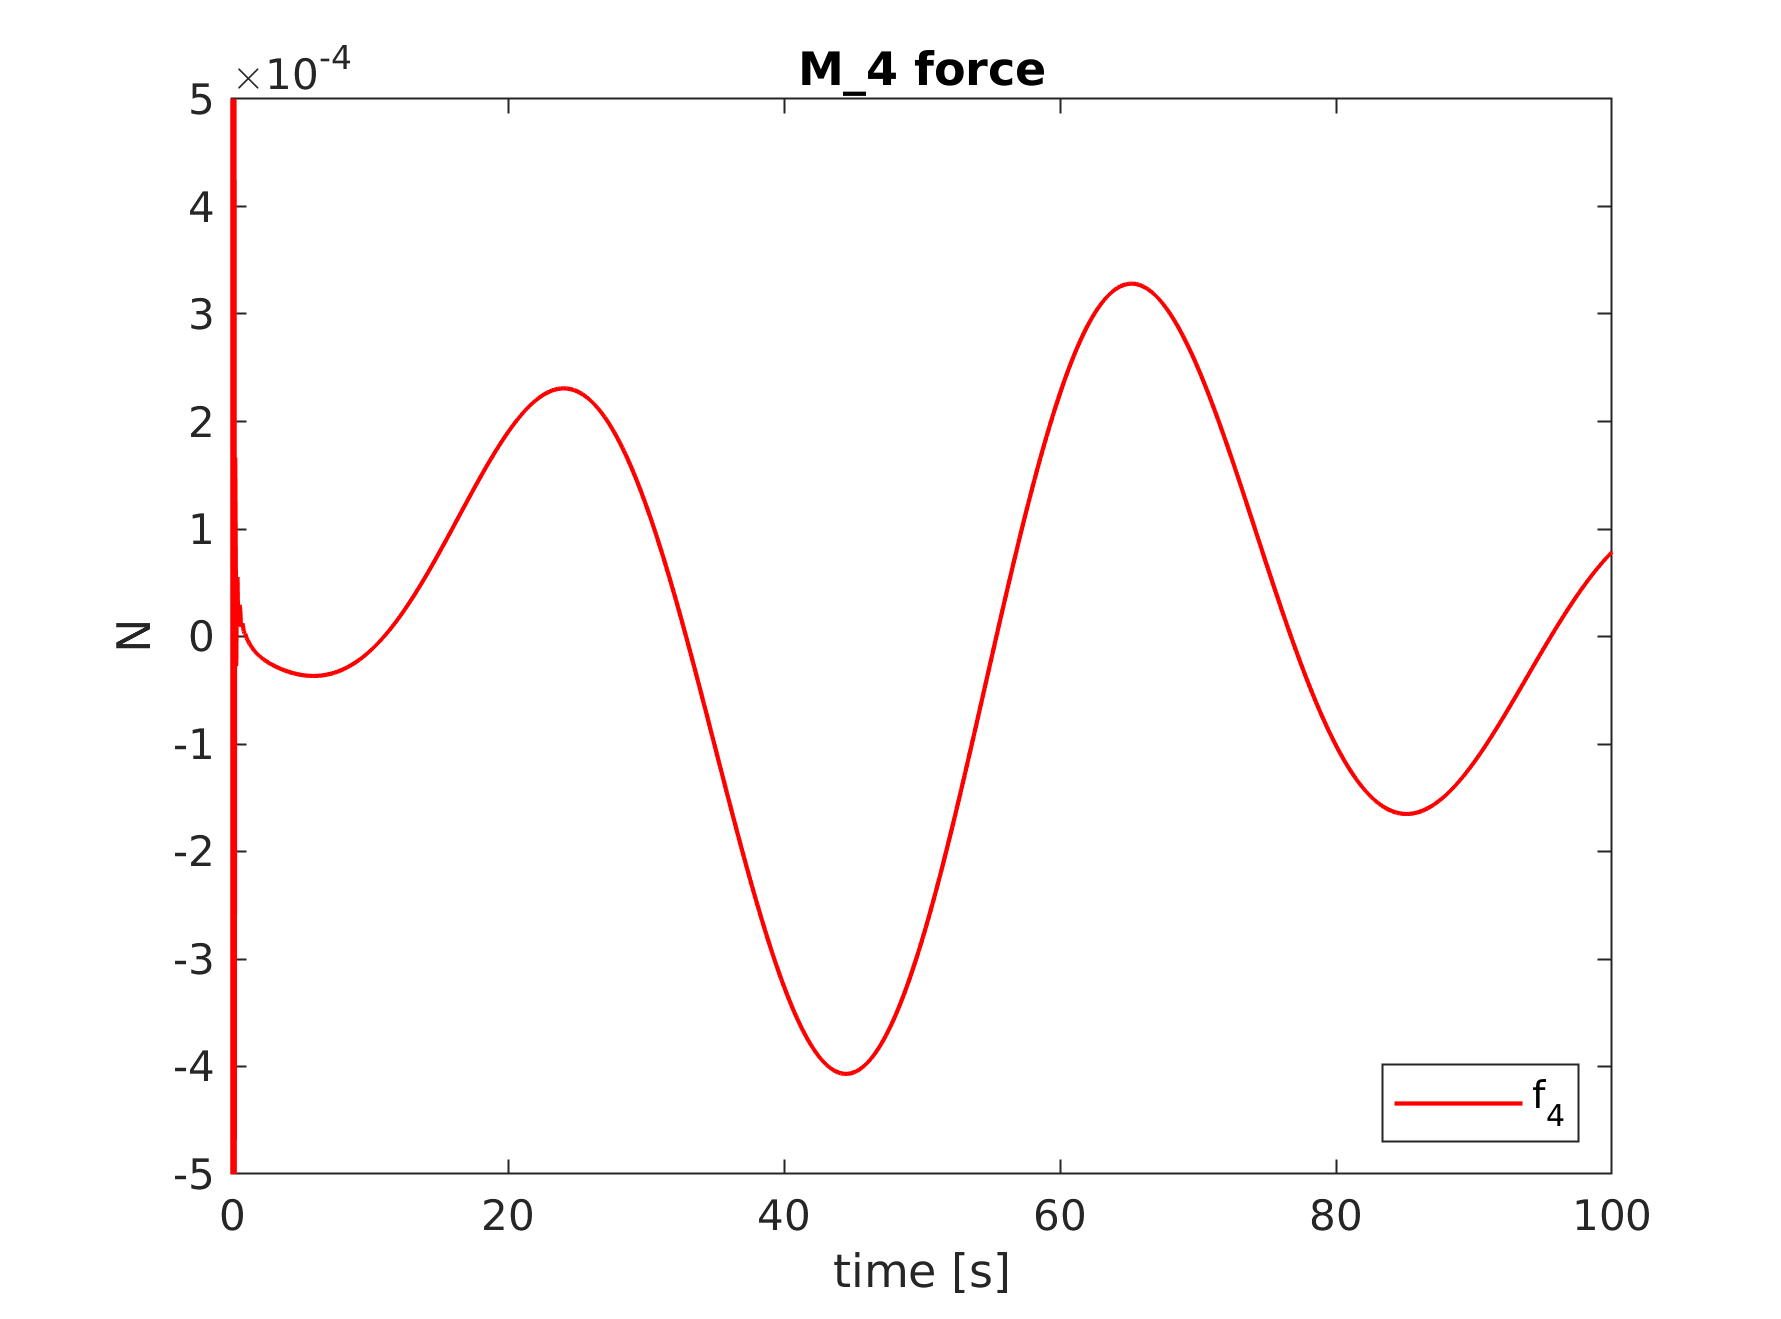
\includegraphics[width=0.7\linewidth]{Images/r4force}
	\caption{Force of rotor n.4.}
	\label{fig:r4force}
\end{figure}


The performances of the double-loop controller decrease when the constraints on motors force saturation are applied. The controller behaves correctly when the vehicle starts with zero error conditions. 

In this case the vehicle follows the vertical trajectory (fig.\ref{fig:positionsetpoint}) and the forces required by the controller are always limited in the boundaries (fig.\ref{fig:forcessetpoint}). The explanation of this behavior is that the quadcopter has an initial small spinning velocity around the equilibrium and by consequence the motor $ \mathcal{M}_4 $ is never activated. The vertical position, instead, is regulated only by motors $ \mathcal{M}_1 $ and $ \mathcal{M}_3 $.

\begin{figure}[H]
	\centering
	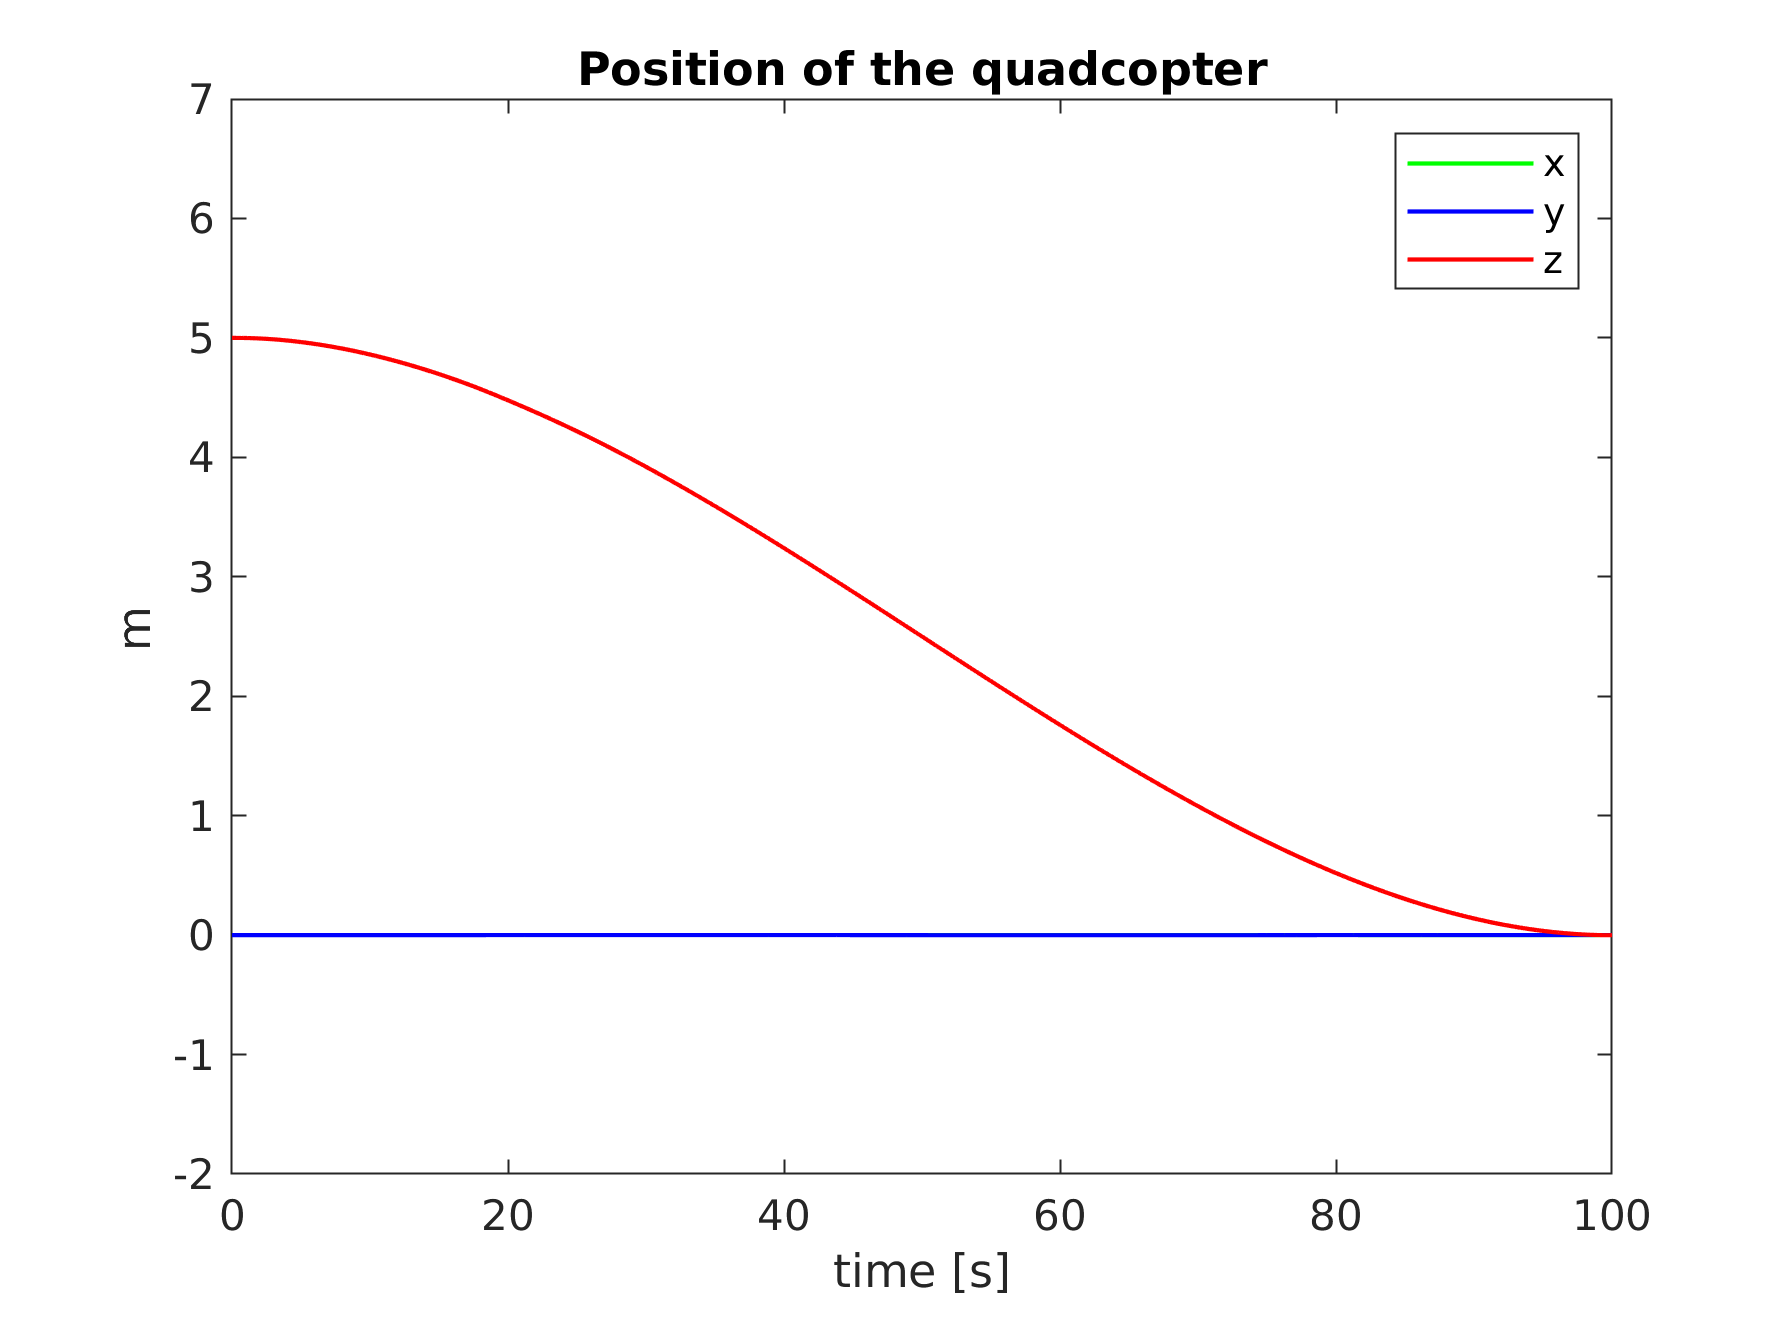
\includegraphics[width=0.7\linewidth]{Images/Position_SetPoint}
	\caption{Position of the quadcopter in Earth frame (force saturation active).}
	\label{fig:positionsetpoint}
\end{figure}

\begin{figure}
	\centering
	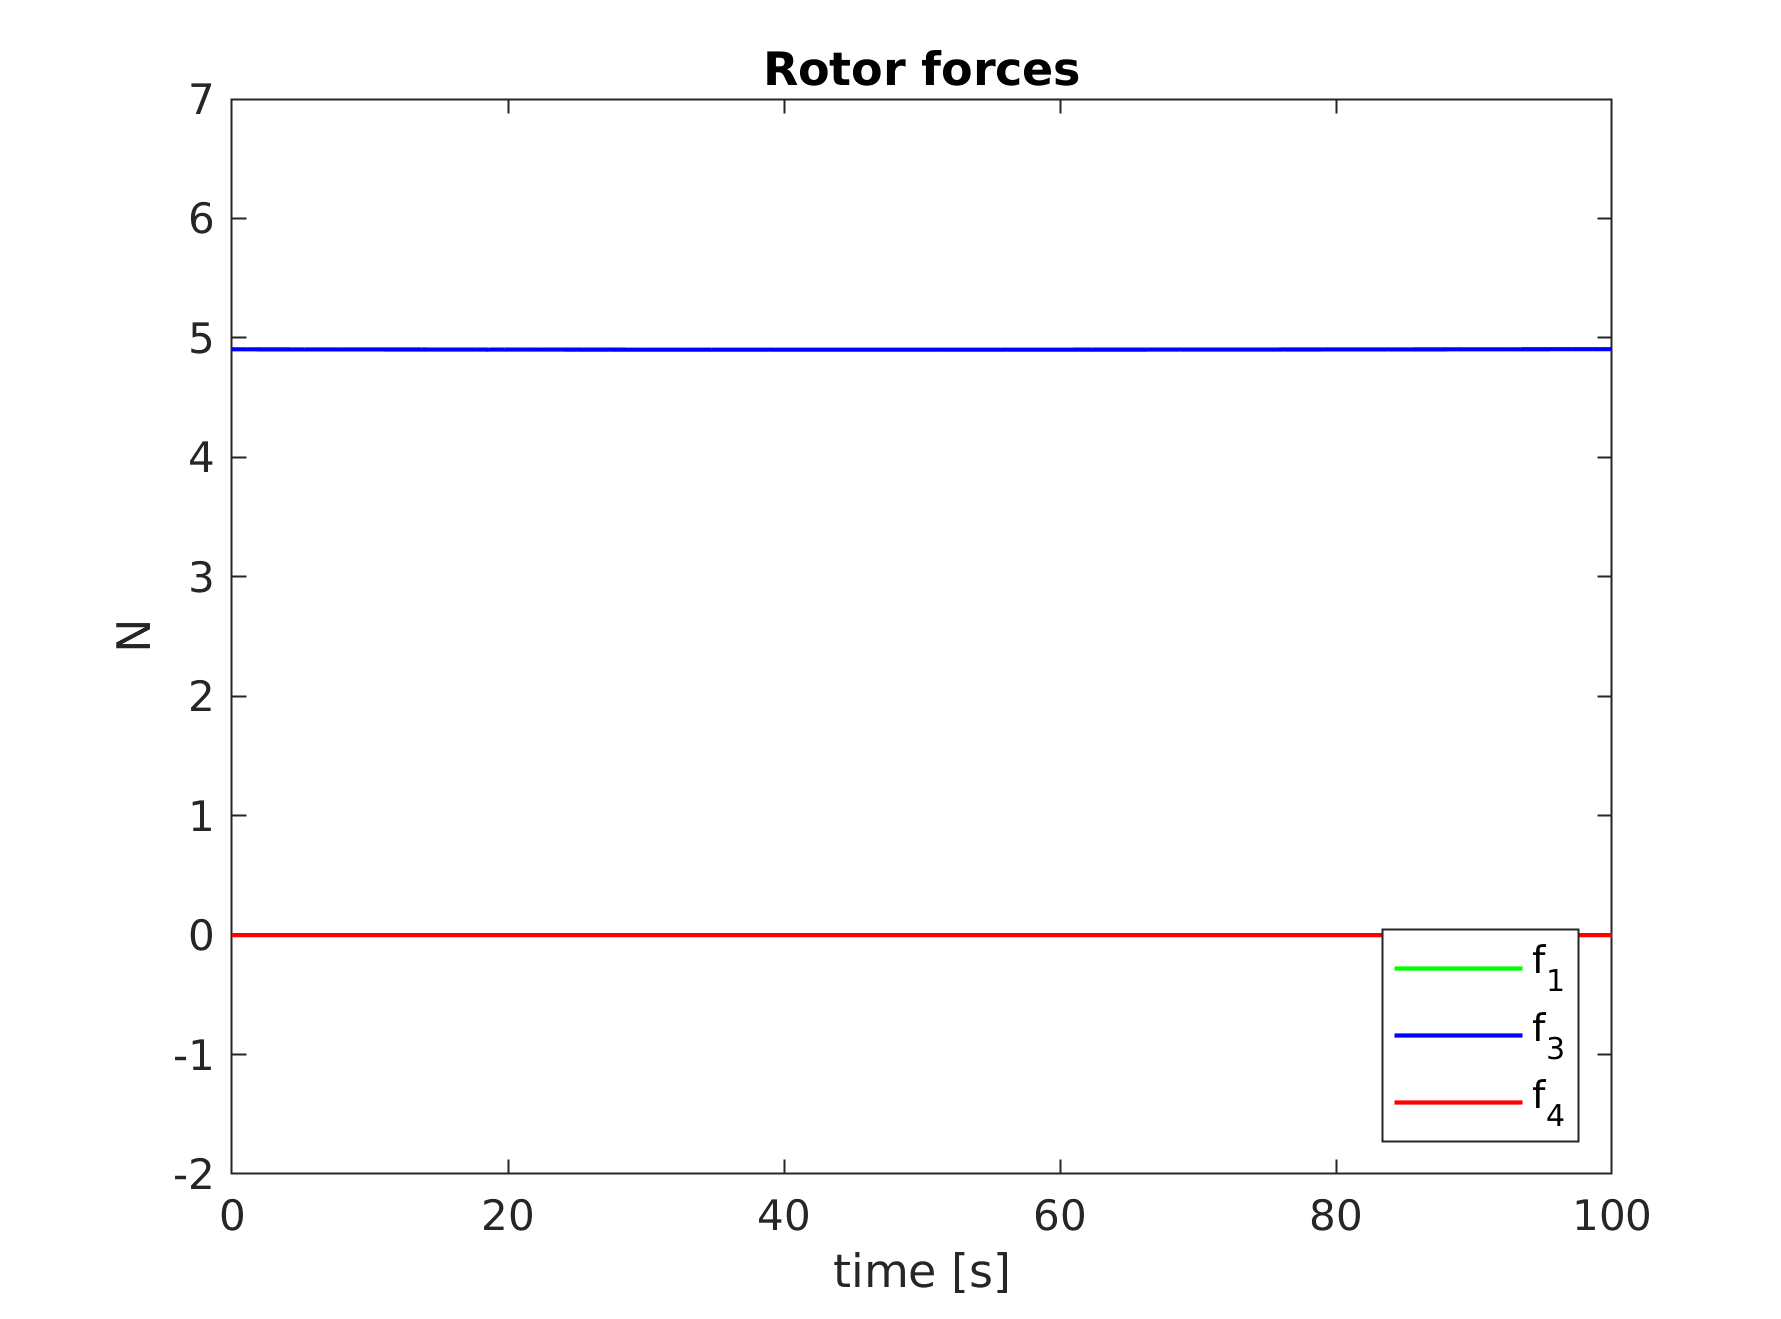
\includegraphics[width=0.7\linewidth]{Images/Forces_SetPoint}
	\caption{Forces required by the double-loop architecture (force saturation active) - only the first 5 seconds.}
	\label{fig:forcessetpoint}
\end{figure}

\section{Conclusions}

In this report we addressed the problem of controlling a quadcopter in case of loss of one of the actuators. The adopted strategy is the use of a double-loop architecture. 

In correspondence of the loss of one input, the state that is chosen to sacrifice is the yaw angle.

The outer control loop is based on a simple linearizing control law. The inner control loop is based on a feedback linearization control law. 

The developed controllers behave appropriately singularly. When interconnected the vertical trajectory is perfectly tracked, while the horizontal position oscillates around the desired one, allowing only slow recovery maneuvers.

Another problem is represented by the motors force saturation: we can consider it as an uncertainty in the model. In this sense, the controller would require a more robust approach as proposed in \cite{lanzon2014flight}. Another solution is to consider saturation in the control design. For example, using an MPC one can introduce constraints relative to reference angle rate in the outer control loop and relative to forces in the inner control loop, and hence obtain inputs satisfying the boundaries imposed.

\clearpage

\bibliographystyle{ieeetr}

\bibliography{sample.bib}

\end{document}

%\begin{center}
%	\begin{tikzpicture}[auto, node distance=2cm,>=latex']
%	
%	% We start by placing the blocks
%	\node [input, name=input] {};
%	\node [sum, below of=input] (sum) {};
%	\node [block, right of=sum] (controller) {Controller};
%	\node [block, right of=controller,
%	node distance=4cm] (system) {System};
%	% We draw an edge between the controller and system block to 
%	% calculate the coordinate u. We need it to place the measurement block. 
%	\draw [->] (controller) -- node[name=u] {$u$} (system);
%	\node [output, right of=system] (output) {};
%	\node [block, below of=u] (measurements) {Measurements};
%	
%	% Once the nodes are placed, connecting them is easy. 
%	\draw [draw,->] (input) -- node {$[\phi_d \\ s] $} (sum);
%	\draw [->] (sum) -- node {$e$} (controller);
%	\draw [->] (system) -- node [name=y] {$y$}(output);
%	\draw [->] (y) |- (measurements);
%	\draw [->] (measurements) -| node[pos=0.99] {$-$} 
%	node [near end] {$y_m$} (sum);
%	\end{tikzpicture}
%\end{center}
